\documentclass[oneside, 12pt, a4paper]{book}

\errorcontextlines=5 % Adjust the number to show more or fewer lines

\makeatletter
\def\input@path{{./templates/}}
\usepackage{thesis_uc3m}
\usepackage{eurosym}
\usepackage{longtable}
\graphicspath{{./figures} {./templates/figures}}
\makeatother

\title{Building a Scalable Parking Management Solution for Multi-Community Deployment}
\author{Andrés Navarro Pedregal}
\degree{Data Science and Engineering and Telecommunication Technologies Engineering}
\graduationyear{2024~--~2025}
\supervisor{David Larrabeiti López}
\placeandyear{Leganés, 2025 \\ Madrid, Spain}

\hypersetup{
  pdfauthor=Andres Navarro Pedregal,
  pdftitle=Final Thesis | Andres Navarro Pedregal | Telecommunication Technologies Engineering,
  pdfsubject=Final Thesis,
  pdfkeywords={Final Thesis, Andres Navarro Pedregal, Telecommunication Technologies Engineering},
}

\addbibresource{./bibliography.bib} % load the bibliography file

\loadglsentries{acronyms} % load the acronyms file

\begin{document}

% \setcounter{tocdepth}{0} % Show only parts and chapters in the table of contents

\frontmatter
\maketitle

\blankpage%
\chapter*{Abstract}

This bachelor thesis presents the design, implementation, and deployment of a distributed parking management system tailored for multi-community environments. The project addresses the growing challenges of urban parking management through an innovative approach that combines edge computing with cloud services.

The system employs a distributed architecture where each community operates autonomously while maintaining centralized oversight. Key components include license plate recognition using machine learning, automated access control, and a web-based management interface. The solution utilizes NVIDIA Jetson Nano devices for edge processing, custom relay boards for hardware control, and AWS cloud infrastructure for centralized management.

The system has been successfully deployed across ten communities in Valencia, Spain, demonstrating its scalability and reliability in real-world conditions. The implementation incorporates robust security measures, including encrypted databases, secure network communications via ZeroTier, and SMS-based user authentication. Environmental challenges, such as the Dana weather event in September 2024, led to system improvements in hardware protection and reliability.

This work contributes to the field of smart city infrastructure by providing a practical, scalable solution for community parking management that balances autonomy with centralized control, setting a foundation for future expansion and enhancement of urban parking solutions.

\textbf{Keywords:} parking management, distributed systems, edge computing, cloud computing, license plate recognition, IoT, smart cities

\blankpage%

\chapter*{Acknowledgments}
\begingroup
\let\clearpage\relax % This temporarily disables \clearpage so the Agradecimientos chapter is on the same page

First and foremost, I would like to express my sincere gratitude to my supervisor, Dr. David Larrabeiti López, for the opportunity to work with him on this project. His guidance, expertise, and support have been invaluable throughout the development of this thesis.

My heartfelt appreciation goes to the Telematics Department of Universidad Carlos III de Madrid, especially to my supervisor again and Dr. José Alberto Hernández Gutiérrez for their unwavering support since the beginning of my academic journey. I am grateful to all members of the department for creating a nurturing and stimulating environment for research and learning.

To ATES, specially Jose Peris for their support and collaboration in the development of the parking management system.

Finally, I would like to thank my colleague Álvaro Ramajo for his collaboration and support throughout this process. Your camaraderie and intellectual contributions have been instrumental in the completion of this thesis.

To all those mentioned and to the many others who have supported me along the way, thank you for your encouragement, patience, and belief in my abilities. This work would not have been possible without you.

\chapter*{Agradecimientos}

En primer lugar, quiero expresar mi más sincero agradecimiento a mi supervisor, el David Larrabeiti López, por la oportunidad de trabajar con él en este proyecto. Su orientación, experiencia y apoyo han sido invaluables durante todo el desarrollo de esta tesis.

Mi más profundo aprecio va para el Departamento de Telemática de la Universidad Carlos III de Madrid, especialmente otra vez a mi supervisor y Dr. José Alberto Hernández Gutiérrez por el apoyo inquebrantable desde el inicio de mi trayectoria académica. Estoy agradecido a todos los miembros del departamento por crear un ambiente estimulante y enriquecedor para la investigación y el aprendizaje.

A ATES, especialmente a Jose Peris por su apoyo y colaboración en el desarrollo de este sistema.

Finalmente, me gustaría agradecer a mi colega Álvaro Ramajo por su colaboración y apoyo durante todo este proceso. Tu camaradería y contribuciones intelectuales han sido fundamentales para la realización de esta tesis.

A todos los mencionados y a los muchos otros que me han apoyado en el camino, gracias por su aliento, paciencia y fe en mis capacidades. Este trabajo no habría sido posible sin ustedes.

\endgroup

\blankpage%

\renewcommand{\contentsname}{Table of Contents}
\tableofcontents

\blankpage%

\listoffigures

\blankpage%

\listoftables

\blankpage%

\printglossary[type=\acronymtype,style=long, title=LIST OF ACROYNMS]

\blankpage%

\mainmatter%

\oldpart{Introduction} % This is the first part, so it is not preceded by a new page

\chapter{Motivation}\label{ch:motivation}

The rapid growth of urban populations and the corresponding increase in vehicle ownership have significantly intensified the challenges associated with parking management in cities worldwide. For instance, the dramatic rise in car usage in Madrid has substantially contributed to heightened levels of environmental pollution \autocite{environmental_impact_madrid_central}. Despite the number of parking spaces in Spain remaining stable between 2014 and 2020 \autocite{urban_mobility_trends}, the escalating demand for parking has resulted in higher costs, prolonged search times, increased traffic congestion, and elevated urban pollution levels.

The inadequacies of traditional, manual \glspl{pms} have further highlighted the need for innovative solutions in this domain. Studies highlight the importance of user-friendly, secure, and reliable systems, with these factors playing a crucial role in influencing parking behavior and preferences \autocite{parking_choices}. Consequently, the development of effective \glspl{pms} remains an essential area of research, particularly as urbanization continues to accelerate.

Advancements in technology provide new opportunities to address these challenges. The proliferation of internet-connected devices, growing by 20\% annually \autocite{iot_growth}, has catalyzed the emergence of \gls{iot}-based \glspl{pms}. These systems aim to mitigate traffic congestion and reduce urban pollution while promoting sustainable and efficient urban mobility. By leveraging real-time data and automation, modern \glspl{pms} offer transformative potential for urban planning and management.

Integrating these advanced systems into urban environments offers multiple benefits, including decreased traffic congestion, reduced pollution, enhanced security, and an improved quality of life for residents. Additionally, \glspl{pms} enable automated parking space management, making them adaptable for a wide range of applications, including urban centers, residential communities, and commercial buildings.

Despite these advancements, the widespread adoption of \glspl{pms} in Spain has faced significant obstacles. Many existing systems rely heavily on human intervention, leading to delays, insufficient information dissemination, and limited control over parking space availability. This dependence on manual operations not only impairs system efficiency but also increases operational costs.

Emerging technologies have inspired the development of innovative \glspl{pms}, such as RFID-based systems \autocite{rfid_smart_parking_management_system}, \gls{iot}-enabled solutions \autocite{development_smart_parking_management_system}, and intelligent parking systems employing image processing techniques \autocite{intelligent_parking_system_image_processing}. However, these systems frequently rely on centralized architectures, which are prone to scalability and reliability issues, particularly during service disruptions. Moreover, many current solutions lack the flexibility needed to accommodate the specific requirements of diverse user groups, limiting their broader applicability.

Addressing these limitations, the primary objective of this project is to design and implement a fully distributed and autonomous \gls{pms} that overcomes the challenges inherent in existing systems. This new approach emphasizes scalability, reliability, and adaptability, with a particular focus on meeting the demands of next-generation smart cities. Through this work, the project aims to contribute to the development of sustainable, efficient, and user-centric parking solutions for urban environments.

\todo{add a graph or somehting to showcase the importance}


\chapter{Statement of the problem}\label{ch:statement_of_problem}

The lack of efficient \glspl{pms} is a pervasive problem in modern cities, exacerbated by the growing number of vehicles and the resulting increase in urban population. Traditional manual \glspl{pms} have proven inadequate in addressing the complexities of modern urban parking, leading to higher costs, longer search times, traffic congestion, and elevated levels of urban pollution. The ongoing development of \glspl{pms} remains a crucial research area, as citizens favor systems that prioritize user-friendliness, security, and reliability \autocite{parking_choices} \autocite{A_Elsonbaty_2020} \autocite{intelligent_parking_system} \autocite{smart_parking_management_system}.

This project aims to address the gap by designing and implementing a fully distributed \gls{pms} tailored for the next generation of smart cities. The proposed system will focus on addressing the inefficiencies and challenges inherent in current \glspl{pms} through a distributed approach that leverages modern technologies. It should be noted that this approach is valid not only for \gls{pms}, but for many other \gls{iot} applications featuring edge computing, sensors, actuators, edge storage and caching.

Given the broad nature of this problem, the scope of this project will be narrowed to a specific environment and use case, as outlined below:

\begin{itemize}
    \item \textbf{Environment:} The system will be designed for urban environments with high vehicle density and limited parking spaces. The case study will focus on a city center with a high volume of vehicles and limited parking availability, reflecting the challenges faced by many modern cities.

    \item \textbf{Atmospheric Conditions:} The system will be designed to operate under typical urban atmospheric conditions, with no specific constraints on temperature, pressure, or humidity. The system will be designed to function in a variety of weather conditions, including rain, heat, and cold.

    \item \textbf{Operational Parameters:} The system will be designed to manage parking spaces in a city center, with a focus on optimizing space utilization, reducing search times, and minimizing traffic congestion. The system will be scalable to accommodate a large number of parking spaces and users.

    \item \textbf{Hardware:} The system will be designed to leverage modern technologies such as \gls{iot} devices, sensors, and cloud computing to provide real-time monitoring and management of parking spaces. The system will be designed to be cost-effective, scalable, and user-friendly.
\end{itemize}


\chapter{Objectives}\label{ch:objectives}

The primary goal of this bachelor thesis is to design and implement a distributed parking management system to address the evolving needs of smart cities. The project aims to overcome the limitations of existing parking management solutions by utilizing scalable and \gls{IoT} technologies. By doing so, it seeks to enhance performance, security, and user experience, contributing to the development of smart city solutions. The specific objectives of the project are outlined below:

\begin{itemize}
	\item \textbf{Analyze Existing Systems:} Review current parking management systems, identifying inefficiencies and challenges. This includes assessing the limitations of centralized systems and understanding the needs of users (drivers and facility managers) to uncover areas for improvement using a distributed approach.

	\item \textbf{Evaluate Relevant Technologies:} Examine key technologies used in parking management systems, focusing on their suitability for a distributed architecture. This involves evaluating \gls{iot} devices, sensors, communication protocols, and data storage methods to determine the most scalable and secure technologies for the proposed system.

	\item \textbf{Design the System Architecture:} Develop the overall design of the distributed parking management system. This includes selecting \gls{iot} sensors, determining data storage solutions, and ensuring that the system can handle high data loads while integrating seamlessly with other smart city systems.

	\item \textbf{System Development:} Implement the system using an agile approach, following best practices in software engineering. This includes iterative planning, design, coding, testing, deployment, and maintenance, with an emphasis on modularity and extensibility to accommodate future updates and integration with emerging technologies (e.g., autonomous vehicles, AI-based traffic management).

	\item \textbf{Evaluate System Performance:} Assess the implemented system's performance based on \glspl{kpi} such as scalability, reliability, data accuracy, and real-time processing capabilities to ensure the system meets its design objectives.

	\item \textbf{Real-World Testing and Validation:} Deploy the system in a real-world urban environment with limited parking capacity. The goal is to validate the system’s effectiveness in managing parking allocation, optimizing resource use, and reducing congestion while testing its robustness, scalability, and performance under actual conditions.

\end{itemize}


\chapter{Document Structure}\label{ch:document_structure}

This thesis is organized into six main parts, each addressing specific aspects of developing a scalable parking management solution for multi-community deployment.

Theoretical Background, \cref{part:theoretical_background}, provides essential knowledge for understanding the technological foundations of the project. It explores cloud computing concepts, including deployment models and service types crucial for system scalability. This part also covers Internet of Things (IoT) technologies, focusing on their architecture, benefits, and challenges in modern applications.

State of the Art, \cref{part:state_of_the_art}, examines the evolution and current state of parking management systems. It traces the historical development of these systems from early mechanical solutions to modern digital implementations. The section on modern trends explores current technologies and approaches in parking management, providing context for the project's innovations.

Methodology, \cref{part:methodology}, forms the core of the thesis, detailing the system's development process. It begins with comprehensive requirements analysis, covering both user and system needs. The design section outlines the system architecture and hardware selections, while the implementation section details the practical realization of the system, including both community-level and cloud components.

Results, \cref{part:results}, presents the outcomes of the project through testing and deployment phases. The testing section covers individual component validation and integrated system testing, while the deployment section discusses the real-world implementation across multiple communities and the challenges encountered.

Conclusions, \cref{part:conclusions}, summarizes the project's achievements and insights. It includes future work recommendations, analysis of the socio-economic impact, and discussion of the regulatory framework governing parking management systems. This part provides a comprehensive overview of the project's implications and potential future developments.

\chapter{Methodological Framework}\label{ch:methodology_approach}

\todo{rewrite to adapt to this project}

To address the research objectives outlined in this thesis, a structured methodological framework is adopted to ensure a comprehensive and rigorous development process. This chapter presents the methodological approach employed in this research, which is grounded in the V-model as established by the \gls{incose} \autocite{INCOSE2015}. The V-model provides a robust framework for project development, facilitating timely and budget-compliant completion through a comprehensive development process.

The methodological framework is composed of seven key stages, each addressing a distinct aspect of the project development process. The stages are designed to ensure clear validation and verification of initial requirements at every stage, guaranteeing that the proposed solution aligns with the project's objectives.

\begin{enumerate}
  \item \textbf{User Requirement Identification}: This stage involves a detailed analysis of the problem statement to identify primary issues and potential solutions. User requirements are defined to ensure that the proposed solution aligns with the project's objectives. This stage is crucial in establishing a clear understanding of the project's scope and requirements.

  \item \textbf{System Design and Architecture}: Based on the identified user requirements, the system architecture is developed, ensuring that the proposed solution is feasible and aligns with the project's objectives. This stage involves a high-level overview of the system components and their interconnections. Requirements are formulated to satisfy the previously defined solution requirements.

  \item \textbf{Component Design and Development}: Building upon the high-level architecture of the solution, a more detailed approach is outlined for each component, taking into account their specific power and data transmission needs. This stage culminates in a comprehensive architecture of the solution, providing a detailed overview of the components, their selection rationale, and their interconnections.

  \item \textbf{Implementation and Manufacturing}: The proposed solution is implemented and manufactured using available tools, integrating the necessary electrical components. This stage includes a detailed description of the implementation process, including the tools and materials used, as well as the integration of electrical components. The development of software and hardware components is also detailed.

  \item \textbf{Component Testing and Verification}: The functionality of each component is verified in a standalone mode, with detailed information provided regarding the verification process. This stage ensures that each component functions as intended, paving the way for system integration.

  \item \textbf{System Testing and Integration}: The methodology for conducting system tests and subsequent analyses is elaborated. System integration is performed by assessing communication between module pairs to ensure that data can be transmitted freely and utilized effectively.

  \item \textbf{Acceptance Testing and Validation}: Validation of the initial requirements is conducted to confirm that all solution requirements have been met. This stage also includes preparations for potential future enhancements, ensuring the solution's scalability and adaptability.
\end{enumerate}

A graphical representation of the V-model is provided in \cref{fig:v_model_methodology} to illustrate the methodology's structure and relationship between the various stages.

\begin{figure}
  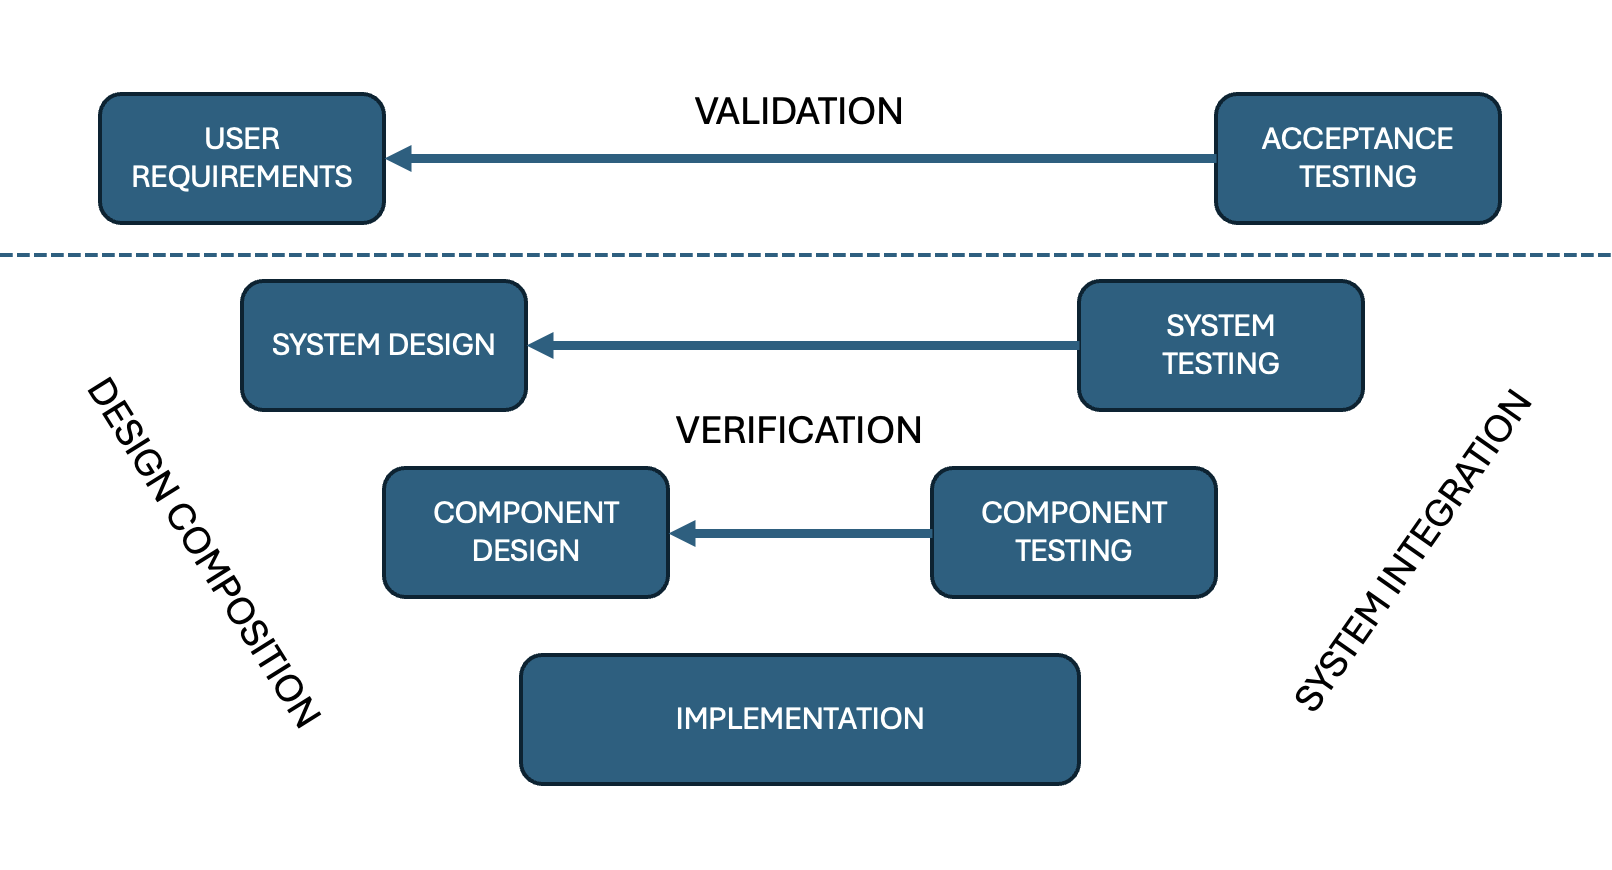
\includegraphics{v_model_methodology.png}
  \caption{Methodological framework based on the V-model from \glsentryshort{incose} with the different stages of the project development process\autocite{ruddle2020vmodel}}\label{fig:v_model_methodology}
\end{figure}

The V-model provides a structured approach to project development, ensuring that all aspects of the project are considered and addressed. By following this methodological framework, this research aims to develop a comprehensive and effective solution for the design and implementation of a fully distributed parking management system tailored for the next generation of smart cities.

% Local Variables:
% jinx-local-words: "incose"
% End:


\oldpart{Theoretical Background}\label{part:theoretical_background}

\chapter{Cloud Computing}\label{ch:cloud_computing}

Cloud computing is a technological paradigm that enables the delivery of computing services, including servers, storage, databases, networking, software, and analytics, over the internet. This model shifts the management of physical infrastructure and resources from on-premises systems to remote data centers managed by cloud service providers. Cloud computing is fundamental to modern digital ecosystems, supporting a wide range of applications from personal use to large-scale enterprise operations.

\section{Definition and Key Concepts}

Cloud computing leverages a network of remote servers hosted on the internet to store, manage, and process data, rather than relying on local computers or private data centers. It offers resources on-demand, enabling users to scale operations according to their needs. The essential characteristics of cloud computing include:

\begin{itemize}
	\item \textbf{On-Demand Self-Service:} Users can access computing resources as needed without requiring human interaction with service providers.
	\item \textbf{Broad Network Access:} Services are accessible over a network, typically the internet, using various devices such as smartphones, tablets, and laptops.
	\item \textbf{Resource Pooling:} Resources are pooled to serve multiple users, ensuring efficiency and scalability.
	\item \textbf{Rapid Elasticity:} Resources can be elastically provisioned and released, enabling scalability according to demand.
	\item \textbf{Measured Service:} Cloud systems automatically control and optimize resource use, charging users based on their consumption.
\end{itemize}

\section{Advantages of Cloud Computing}

The adoption of cloud computing offers several advantages that have contributed to its widespread popularity. One of the most significant benefits is its scalability and flexibility. Cloud computing enables organizations to adjust their resource usage dynamically based on real-time needs, eliminating the need for over-provisioning and supporting workloads of varying demands effectively. This adaptability ensures that resources are utilized efficiently, minimizing waste and optimizing performance.

Cost efficiency is another critical advantage. By using cloud services, organizations can avoid the significant capital expenditures associated with purchasing and maintaining hardware and software. Instead, they incur operational costs only for the resources they consume, making cloud computing an economically viable solution for businesses of all sizes. Additionally, cloud computing enhances accessibility and collaboration. Since cloud-based applications and services are accessible from anywhere with an internet connection, distributed teams can collaborate seamlessly, a feature that has become indispensable in today’s increasingly globalized and remote work environments.

Reliability is also a key strength of cloud computing. Leading cloud providers ensure high levels of availability by deploying redundant systems across geographically dispersed data centers, thereby minimizing downtime and enhancing disaster recovery capabilities. Furthermore, security is a paramount concern addressed by cloud providers. They invest significantly in advanced measures such as encryption, firewalls, and regular security audits, ensuring robust protection against cyber threats and unauthorized access. These combined advantages make cloud computing a transformative technology, supporting innovation and operational efficiency in diverse sectors.

\section{Types of Cloud Computing}

Cloud computing services are categorized into different types based on their deployment models and the services they provide. These distinctions allow organizations to select a cloud strategy that aligns with their specific requirements.

\subsection{Deployment Models}

\begin{itemize}
	\item \textbf{Public Cloud:} A public cloud is owned and operated by third-party providers, delivering resources over the internet. Examples include \gls{aws}, Microsoft Azure, and Google Cloud Platform. It offers cost-effectiveness and scalability but may pose data sovereignty concerns for certain organizations.
	\item \textbf{Private Cloud:} A private cloud is used exclusively by a single organization. It offers greater control over data and infrastructure, making it suitable for industries with strict regulatory requirements.
	\item \textbf{Hybrid Cloud:} A hybrid cloud combines public and private cloud environments, enabling organizations to benefit from both scalability and control. This model is particularly useful for balancing workloads and maintaining sensitive data on-premises while leveraging the public cloud for other operations.
	\item \textbf{Multi-Cloud:} A multi-cloud strategy involves using multiple cloud providers to mitigate risks associated with vendor lock-in and enhance reliability and performance.
\end{itemize}

\subsection{Service Models}

Cloud computing services are typically offered in the following models:

\begin{itemize}
	\item \textbf{\gls{iaas}:} Provides virtualized computing resources over the internet, including servers, storage, and networking. Users manage operating systems and applications while the provider handles the infrastructure.
	\item \textbf{\gls{paas}:} Offers a platform that includes hardware, software, and development tools to build, test, and deploy applications. It abstracts the complexities of infrastructure management, enabling developers to focus on coding.
	\item \textbf{\gls{saas}:} Delivers software applications over the internet on a subscription basis. Users can access the software through a browser without worrying about installation or maintenance.
\end{itemize}

\chapter{Internet of Things}\label{iot}

The \gls{iot} is a paradigm that establishes a network of interconnected devices equipped with sensors, software, and communication technologies. This enables seamless interaction between the physical and digital realms, facilitating the collection, transmission, and processing of data. Through its ability to deliver enhanced functionality and automation, the \gls{iot} has numerous applications, particularly in smart city infrastructure. These applications span healthcare, transportation, energy management, and urban planning.

The main point of \gls{iot} is its capacity for interconnectivity, enabling devices to autonomously communicate and share data. Advanced sensing technologies augment this connectivity, capturing real-world metrics such as temperature, motion, or occupancy. The processing of the data is achieved through edge computing, which provides localized analysis, or cloud computing for centralized processing, tailored to meet latency and scalability demands. This processed data is subsequently integrated with actuators, enabling automation of tasks such as the management of parking space access without requiring human intervention.

\section{Architecture of IoT Systems}
The architecture of \gls{iot} systems is structured across four principal layers. The perception layer constitutes sensors and actuators, which interface directly with the physical environment to gather data and execute specific actions. Data transmission occurs within the network layer, leveraging communication protocols such as Wi-Fi, Bluetooth, or cellular networks. The processing layer transforms raw data into actionable insights through edge or cloud computing methodologies. Finally, the application layer provides interfaces for end-users, ensuring an intuitive and accessible experience tailored to diverse functionalities.

\section{Benefits of IoT}
The adoption of \gls{iot} technologies confers significant advantages across multiple sectors, particularly in the realm of parking management systems. Real-time monitoring capabilities, enabled by sensors, deliver continuous updates on parking space availability, reducing search times and alleviating urban congestion. Automation, facilitated by actuators, streamlines operations such as access control and reservation management, minimizing human intervention. Moreover, \gls{iot}-driven data analytics empower urban planners with insights to optimize resource allocation and develop informed policies. The energy efficiency inherent in smart systems aligns with sustainability objectives by curbing unnecessary resource consumption.

\section{Challenges and Limitations}
The deployment of \gls{iot} systems presents several challenges. Scalability remains a critical concern, particularly in large-scale implementations like city-wide parking systems. The management of sensitive information collected by \gls{iot} devices necessitates data security and privacy measures to itigate risks. Interoperability challenges, stemming from disparate manufacturer standards and communication protocols, complicate system integration.



\oldpart{State of the art}\label{part:state_of_the_art}

\chapter{Historical Development}\label{ch:historical_development}

In the early 20th century, as urbanization accelerated and automobile ownership increased, the need for efficient parking solutions became apparent. The first significant step in this direction came in 1905 with the Garage Rue de Ponthieu \autocite{mcdonald2005parking} in Paris, designed by Auguste Perret. This multi-story concrete structure, see \cref{fig:garage_rue_de_ponthieu}, featured internal elevators to transport cars between floors, where attendants would manually park them. While not fully automated, this innovation laid the foundation for future parking systems by maximizing vertical space utilization.

The 1920s marked the beginning of more advanced parking solutions, particularly in major U.S. cities. The Paternoster system \autocite{paternoster2022}, resembling a Ferris wheel for cars, refer to \cref{fig:pater_noster_parking_system}, could accommodate eight vehicles in the space typically used for two. This period also saw the introduction of Kent Automatic Garages in New York in 1928, which employed an electric "parker" to lift and move cars to available spaces. These early automated systems represented significant progress in addressing the growing demand for parking in densely populated urban areas.

\begin{figure}
	\hfill
	\begin{subfigure}{0.45\textwidth}
		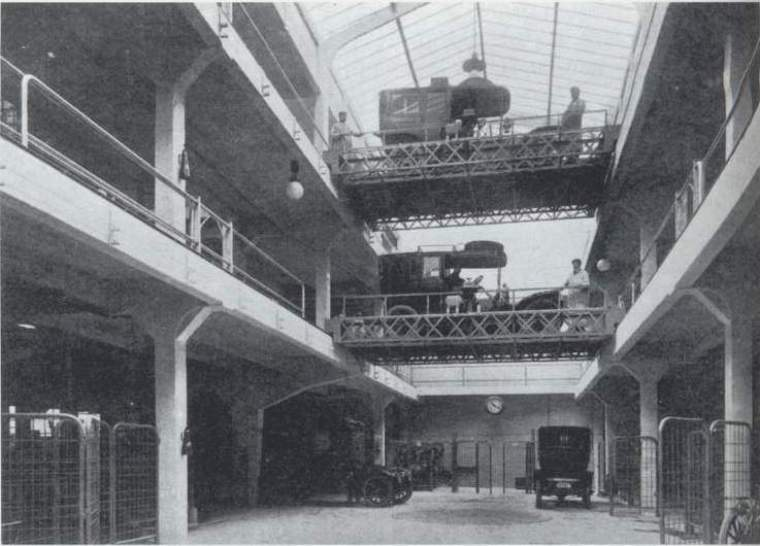
\includegraphics{garage_du_rue_ponthieu.jpg}
		\caption{Garage Rue de Ponthieu in Paris, 1905 \autocite{mcdonald2005parking}.}\label{fig:garage_rue_de_ponthieu}
	\end{subfigure}
	\hfill
	\begin{subfigure}{0.45\textwidth}
		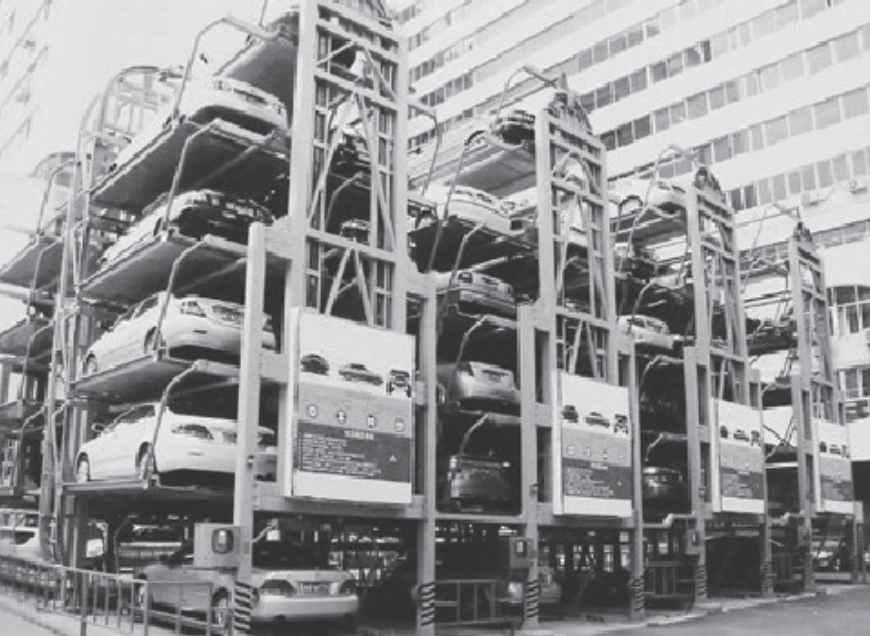
\includegraphics{paternoster.png}
		\caption{Paternoster system, 1920s \autocite{paternoster2022}.}\label{fig:pater_noster_parking_system}
	\end{subfigure}
	\hfill

	\caption{Historical developments in parking management systems.}
\end{figure}

The 1930s brought another crucial development with the introduction of parking meters, revolutionizing on-street parking management. This innovation allowed cities to better regulate parking durations and generate revenue from public parking spaces. The subsequent decades, particularly the 1940s and 1950s, witnessed a surge in the development of automated parking systems in the United States, with designs such as Bowser, Pigeon Hole, and Roto Park \autocite{shoup2012cars} gaining popularity.

While interest in automated parking systems temporarily waned in the U.S. during the 1960s to 1980s, development continued in Europe and Asia. Notable advancements included the Auto Stacker system in London in 1961 and Wohr's Electromechanical Parking System Type 100 \autocite{hardingaps2021history} in Germany in 1962. During this period, Japan emerged as a leader in automated parking systems, with significant growth continuing into the 1990s.

The late 20th century marked the beginning of the digital revolution in parking management. The 1990s saw the introduction of parking guidance systems, which used sensors to monitor occupancy and provide real-time information to drivers. This technology significantly reduced the time and frustration associated with finding available parking spaces in large facilities.

The early 2000s ushered in a new era of smart parking solutions. In 2002, the first robotic parking garage in the United States opened in Hoboken, New Jersey \autocite{usatoday2007robotic}, showcasing the potential of fully automated parking facilities. This period also saw the rapid development of technologies such as license plate recognition systems, mobile parking apps for finding and reserving spaces, and IoT-based parking management systems.

In recent years, parking management systems have continued to evolve, incorporating advanced technologies such as artificial intelligence and machine learning for predictive parking analytics. Cloud-based parking management platforms have become increasingly common, offering scalable and flexible solutions for parking operators. Furthermore, the integration of parking systems with broader smart city initiatives and connected vehicle technologies is paving the way for more efficient and sustainable urban mobility solutions.

The evolution of parking management systems reflects broader technological trends, moving from mechanical solutions to digital, interconnected systems. Today's parking management solutions prioritize efficiency, user experience, and environmental sustainability, addressing not only the immediate needs of drivers and parking operators but also contributing to the broader goals of smart urban planning and reduced environmental impact.

As cities continue to grow and evolve, parking management systems will undoubtedly play a crucial role in shaping the future of urban mobility. The ongoing development of these systems promises to further optimize space utilization, reduce traffic congestion, and enhance the overall urban experience for residents and visitors alike.

\chapter{Modern Trends}\label{ch:modern_trends}

Automated parking management systems have evolved significantly to address the unique needs of residential communities. Currently, various types and technologies are employed in modern parking management solutions, focusing on their application in community settings. Sensor-based systems utilize advanced sensing technologies, such as ground sensors embedded in pavement and overhead sensors mounted above parking spaces, to monitor and manage parking spaces efficiently. These sensors provide real-time data on occupancy, enabling efficient space utilization and reducing search times for residents.

\gls{lpr} systems have gained popularity in community parking management, offering advantages such as automated access control, visitor management, and enforcement of parking regulations. \gls{rfid} technology provides another efficient solution, particularly beneficial for large residential complexes with multiple parking areas. Mobile application-integrated systems offer residents a user-friendly interface to interact with the parking system, providing features like real-time availability information, digital permits, and reservation capabilities.

Cloud-based management platforms have revolutionized parking management by offering centralized, scalable solutions with real-time data analytics, remote management capabilities, and enhanced security. Smart gate systems, integrated with other parking management technologies, form a crucial component of modern community parking solutions, enhancing security and ensuring smooth traffic flow.

The choice of parking management system for a residential community depends on factors such as the size of the community, budget constraints, and specific parking challenges. Often, a combination of these technologies is employed to create a comprehensive, efficient, and user-friendly parking management solution tailored to the unique needs of each community. As urban populations continue to grow and vehicle ownership increases, these advanced parking management systems will play an increasingly important role in optimizing space utilization, improving resident satisfaction, and contributing to more sustainable urban environments.


\oldpart{Methodology}\label{part:methodology}

\chapter{Requirements}\label{ch:requirements}

The \gls{pms} for this project is designed to address the evolving needs of various users, including parking facility managers and drivers. The system's primary objective, detailed in \cref{ch:objectives}, is to overcome the limitations of traditional parking management systems by improving scalability, reliability, and user adaptability, while aligning with the goals of smart city initiatives.

To achieve this, user and system requirements are identified. These requirements are essential for ensuring the system’s effectiveness, efficiency, and alignment with the diverse needs of its users. The system's technical and functional specifications are also established to ensure its successful implementation.

\section{User Requirements}\label{sec:user_requirements}

The user requirements for the distributed \gls{pms} are determined through a thorough analysis of the needs and expectations of parking facility managers. These requirements are critical for designing a system that effectively addresses operational challenges, improves the efficiency of parking space utilization, and integrates seamlessly into existing urban mobility frameworks.

The primary users of the system, parking facility managers and drivers, have specific needs that the system is designed to meet. Their main objectives include improving parking management efficiency, ensuring the safety of the parking environment, and optimizing space utilization across multiple facilities. The system needs to enable them to monitor parking space availability in real-time, manage entry and exit of vehicles, and provide essential data for decision-making and reporting.

The requirements for the users can be broken down into the following key areas:

\subsection{Real-Time Monitoring and Management}

Parking facility managers need a system that provides real-time monitoring of parking spaces. This feature is essential for ensuring that parking spaces are used efficiently and that any underutilized spaces are identified and optimized. Real-time data to track the occupancy status of each parking spot, which is crucial for streamlining operations, reducing congestion, and improving the overall customer experience.

The system also allows parking facility managers to retrieve occupancy patterns and identify peak demand times, which helps adjust pricing strategies, optimize space allocation, and ensure parking spaces are available when needed.

\subsection{Automation of Parking Access}

Automation is another key requirement for the parking management system. Parking facility managers need a system that controls vehicle access to parking areas without requiring human intervention. Automated gates and barriers are essential for improving efficiency, reducing delays, and ensuring that vehicles can enter and exit parking facilities smoothly. These automated systems are integrated with real-time monitoring data to ensure that only authorized vehicles can access specific parking areas.

The system also provides tools for managing access rights based on specific criteria, such as license plate, membership status, or occupancy. Parking facility managers need to configure access control rules and monitor the effectiveness of these rules in real-time.

\subsection{Security and Incident Management}

Ensuring the security of parking facilities is a critical concern for parking facility managers. The system needs to incorporate security features to prevent unauthorized access to parking areas, detect potential security breaches, and provide timely alerts for incidents such as unauthorized parking or other violations. While surveillance systems are removed from the technical specifications, the cameras used for real-time monitoring still play a role in incident detection, as they capture images or video that can be reviewed in the event of an issue.

Real-time alerts are required for events such as access attempts by unauthorized vehicles, security breaches, or potential hazards. These alerts are sent to parking facility managers through the system's notification mechanisms, allowing them to respond quickly and effectively to incidents.

\subsection{Data Analytics and Reporting}

Parking facility managers need access to detailed reports and analytics on parking usage, including occupancy rates, peak demand times, revenue generation, and space utilization patterns. The system provides the ability to download the user data to peform reports, assisting in operational planning, resource allocation, and decision-making.

\section{System Requirements}\label{sec:system_requirements}

To meet the diverse user requirements, the distributed \gls{pms} is designed with several key system requirements in mind. These requirements focus on ensuring that the system is scalable, reliable, secure, and user-friendly, while also supporting the goals of smart city initiatives.

The main system requirements are as follows:

\subsection{Real-Time Monitoring}

The system needs to incorporate cameras for monitoring parking space occupancy in real-time. These cameras must be accurate, reliable, and capable of detecting vehicle presence or absence in parking spaces. The system must be able to process data from numerous cameras across multiple locations simultaneously, ensuring that the information provided to parking facility managers is accurate and timely.

Furthermore, the camera-based monitoring system must be robust enough to handle environmental factors such as weather conditions and lighting variations.

\subsection{Automation and Access Control}

Automated gate and barrier systems are a critical component of the system. These systems must be fully integrated with the parking management platform, allowing for real-time updates on space availability and enabling seamless access control. Vehicles must be able to enter and exit parking facilities autonomously based on the available space data, without the need for human intervention.

Access control mechanisms also need to ensure that only authorized vehicles can enter restricted areas. This can include integration with \gls{lpr} systems, RFID-based solutions, or mobile applications that validate the identity of the vehicle and its access privileges.

\subsection{Scalability and Flexibility}

The system architecture needs to be scalable and flexible to accommodate a growing number of parking facilities, users, and devices. As demand for parking management grows, the system must be able to scale horizontally, adding additional cameras, sensors, or access control systems without impacting performance. Moreover, the system must be modular, allowing for easy updates or integration of new features.

\subsection{Security and Availability}

Given the importance of the system in managing urban mobility and infrastructure, security and availability are paramount. The system must be resilient to cyberattacks and other threats, with multiple layers of security in place to protect sensitive data and ensure continuous availability of services. Redundancy mechanisms, such as backup servers and data replication, are required to ensure high availability and minimize service interruptions. The system must be capable of maintaining operations even in the event of network outages or hardware failures. Interoperability is also a key consideration. The system must be designed to work seamlessly with existing infrastructure and technologies, both within the parking facilities and within the broader smart city ecosystem.

\subsection{Physical System Requirements}

In terms of hardware, the parking management system requires a robust and reliable physical infrastructure to support the real-time monitoring and automation functions. This infrastructure includes:

\begin{itemize}
	\item \textbf{Cameras:} High-resolution cameras capable of detecting vehicle occupancy in parking spaces. These cameras must be weather-resistant, durable, and equipped with night vision or infrared capabilities to ensure reliable performance in various environmental conditions, such as low light or harsh weather.
	\item \textbf{Gate and Barrier Systems:} Automated gates and barriers for controlling vehicle access to parking areas. These systems must be seamlessly integrated with the overall parking management system to allow for real-time updates on space availability and facilitate the automated entry and exit of vehicles.
	\item \textbf{Network Infrastructure:} A robust communication system to transmit data from cameras, sensors, and access control devices to central servers. The network infrastructure must support high-speed data transfer and be resilient to failures.
\end{itemize}

The physical infrastructure must be designed for scalability and ease of maintenance, allowing for the expansion or upgrade of components as needed.

\subsection{Data Privacy and Storage}

Data privacy and security are paramount concerns in the design of the parking management system. The system must comply with relevant data protection laws, such as the \gls{gdpr} \autocite{gdpr}, to safeguard personal information and prevent unauthorized access to sensitive data.

The data collected by the system, including parking history, vehicle entry and exit times, and payment details, must be encrypted both during transmission and while stored in the system’s databases. Key data privacy and storage requirements include:

\begin{itemize}
	\item \textbf{Secure Storage:} All personal and parking-related data should be stored in secure, encrypted databases with access restricted to authorized personnel only.
	\item \textbf{Data Retention:} The system must adhere to strict data retention policies, ensuring that data is stored only for the minimum time necessary to fulfill the purpose of the service, in accordance with relevant privacy regulations.
	\item \textbf{User Consent:} The system must obtain explicit consent from users for data collection, explaining the types of data collected and how it will be used, stored, and shared.
	\item \textbf{Access Control:} The system must include role-based access control mechanisms to ensure that only authorized personnel can access sensitive data, and it must provide audit logs to track data access and modifications.
\end{itemize}

In addition to ensuring compliance with privacy regulations, the system must include robust mechanisms for data breach detection and response, ensuring that any unauthorized access or data compromise is identified and addressed promptly.

\chapter{Design}\label{ch:design}

The proposed parking management system employs a distributed architecture combining edge computing with cloud services, designed to meet the functional requirements outlined in \ref{ch:requirements}. The solution adopts a distributed architecture that combines edge computing capabilities in local terminals with cloud-based interfaces, achieving an optimal balance between responsiveness and scalability.

\section{System Architecture}

The architecture of the system is divided into three main subsystems: the license plate recognition system, the back-end system, and the front-end system. Each subsystem plays a distinct role in ensuring the overall functionality and efficiency of the parking management solution.

The \textbf{license plate recognition system} is responsible for detecting vehicles and identifying their license plates. This subsystem utilizes advanced image processing techniques to extract license plate information from live video feeds. By processing this data locally at the edge, the system minimizes latency and ensures real-time responsiveness. The design emphasizes modularity to facilitate future upgrades or integration with other recognition technologies.

The \textbf{back-end system} serves as the central hub for data processing and logic management. It handles user authentication, license plate management, and communication with both the front-end interface and physical access control mechanisms. The back-end is also tasked with orchestrating requests from users, such as granting or denying access based on predefined rules. Additionally, it interfaces with community-specific terminals to control garage door operations securely and efficiently.

The \textbf{front-end system} provides an intuitive interface for end-users to interact with the parking management solution. Designed with usability in mind, it allows users to perform essential tasks such as registering new license plates, monitoring parking events, and remotely opening garage doors. The front-end is accessible via web browsers and mobile applications, ensuring seamless interaction across diverse platforms.

Each of these subsystems is described in more detail below to illustrate their roles within the overall architecture.

\subsection{License Plate Recognition System}

The license plate recognition system is a critical component of the parking management solution. Its primary function is to identify vehicles by analyzing video streams captured at entry and exit points. This subsystem consists of two main elements: a camera for capturing video footage and a computational unit for processing these images.

The camera continuously monitors designated areas near garage doors to detect approaching vehicles. Once a vehicle is detected, the computational unit processes the video feed to extract license plate information using machine learning algorithms optimized for accuracy and speed. The extracted data is then transmitted to the back-end system for further validation.

This design ensures that license plate detection operates independently within each community terminal, reducing reliance on external servers and enhancing fault tolerance.

\subsection{Back-End System}

The back-end system acts as the brain of the parking management solution. Its responsibilities include managing user accounts, storing license plate data securely, and processing requests from both users and community terminals.

A key feature of this subsystem is its ability to work autonomously without requiring any external services, in case of errors with the external services or connection interruptions. By adopting this architecture, it ensures that each community operates autonomously while still benefiting from centralized oversight when required.

The back-end also integrates with physical access control systems to enable automated garage door operations. For instance, upon receiving a valid access request from the Licence Plate Recognition System or user interface, it triggers the appropriate mechanism to open or close garage doors.

To ensure scalability and reliability, the back-end is deployed on each specific community terminal, allowing it to handle local requests efficiently. This distributed architecture minimizes latency and enhances system responsiveness, even under heavy loads.

\subsection{Front-End System}

The front-end system functions as the primary interface between users and the parking management solution, offering an intuitive and accessible platform for interaction. Its design emphasizes simplicity and usability, transforming complex operations into seamless workflows.

Through this interface, users can perform essential tasks such as registering or removing license plates, monitoring real-time parking availability, accessing detailed logs of parking events, and remotely controlling garage doors within authorized communities. The system is designed to be universally accessible, supporting both desktop browsers and mobile devices to ensure convenience across various platforms.

Security is a fundamental aspect of the front-end system, with all communications between the user interface and the back-end encrypted using industry-standard protocols. Additionally, role-based access controls are implemented to restrict sensitive operations to authorized personnel, further enhancing the system's security and reliability.

\section{Hardware}

The hardware section of this project focuses on the essential components required for the effective operation of the parking management system. The selected hardware includes terminals, cameras, and a server, each playing a critical role in ensuring the system's functionality and efficiency.

A comprehensive study was conducted to identify the most budget-friendly hardware options that still meet the necessary requirements for performance and reliability. This analysis took into account factors such as cost, durability, and compatibility with the overall system architecture. The goal was to strike a balance between affordability and capability, ensuring that the chosen hardware would effectively support the project's objectives while remaining economically viable for deployment across multiple communities.

\subsection{Terminals}\label{subsec:design_terminal}

The terminals are the core part of the deployment and is where all the processing is done to manage each community. In order to provide the necessary capabilities for the community such as opening the garage doors and detecting the cars. For that, the requirements of the terminals are that it must support Linux operating system to be able to run the programs, and als it must be able to have the necessary computing capacity to run the \gls{ml} programs to detect the licence plates. In order to select the correct computer, different alternatives are studied, shown in \cref{tab:sbc-comparison}.

\begin{longtable}{|l|c|}
	\hline

	% Jetson Orin Nano
	\multicolumn{2}{|c|}{\textbf{NVIDIA Jetson Orin Nano}}                    \\
	\hline
	CPU       & 6-core Arm Cortex-A78AE                                       \\
	CPU Clock & 1.5 GHz                                                       \\
	GPU       & 1024-core NVIDIA Ampere                                       \\
	RAM       & 8GB LPDDR5                                                    \\
	USB Ports & 3x USB 3.2 Gen2, 3x USB 2.0                                   \\
	Ethernet  & 1x Gigabit Ethernet                                           \\
	Wi-Fi     & Not specified                                                 \\
	Bluetooth & Not specified                                                 \\
	Power     & 7W - 15W                                                      \\
	Price     & 600 \euro                                                     \\
	\hline

	% Jetson Nano
	\multicolumn{2}{|c|}{\textbf{NVIDIA Jetson Nano}}                         \\
	\hline
	CPU       & Quad-core Arm A57                                             \\
	CPU Clock & 1.43 GHz                                                      \\
	GPU       & 128-core Maxwell                                              \\
	RAM       & 4GB LPDDR4                                                    \\
	USB Ports & 4x USB 3.0, 1x USB 2.0                                        \\
	Ethernet  & Gigabit Ethernet                                              \\
	Wi-Fi     & 802.11ac                                                      \\
	Bluetooth & Bluetooth 5.0                                                 \\
	Power     & 5W / 10W                                                      \\
	Price     & 220 \euro                                                     \\
	\hline

	% Raspberry Pi 4
	\multicolumn{2}{|c|}{\textbf{Raspberry Pi 4}}                             \\
	\hline
	CPU       & Quad-core Arm Cortex-A72                                      \\
	CPU Clock & 1.5 GHz / 1.8 GHz                                             \\
	GPU       & VideoCore VI                                                  \\
	RAM       & 1GB/2GB/4GB/8GB LPDDR4                                        \\
	USB Ports & 2x USB 3.0, 2x USB 2.0                                        \\
	Ethernet  & Gigabit Ethernet                                              \\
	Wi-Fi     & 802.11ac (2.4 GHz and 5.0 GHz)                                \\
	Bluetooth & Bluetooth 5.0                                                 \\
	Power     & 5V DC via USB-C (3A)                                          \\
	Price     & 87 \euro                                                      \\
	\hline

	% Raspberry Pi 5
	\multicolumn{2}{|c|}{\textbf{Raspberry Pi 5}}                             \\
	\hline
	CPU       & Quad-core Arm Cortex-A76                                      \\
	CPU Clock & 2.4 GHz                                                       \\
	GPU       & VideoCore VII                                                 \\
	RAM       & 4GB/8GB LPDDR4X                                               \\
	USB Ports & 2x USB 3.0, 2x USB 2.0                                        \\
	Ethernet  & Gigabit Ethernet                                              \\
	Wi-Fi     & 802.11ac (2.4 GHz and 5.0 GHz)                                \\
	Bluetooth & Bluetooth 5.0                                                 \\
	Power     & 5V/5A DC power (USB-C PD)                                     \\
	Price     & 125 \euro                                                     \\
	\hline

	\caption{Comparison of Single-Board Computers} \label{tab:sbc-comparison} \\
\end{longtable}

For this project, the NVIDIA Jetson Nano is used due to the advanced GPU and the relative cheap price-point compared to the NVIDIA Jetson Orin Nano. Moreover, the Jetson Nano is able to run the \gls{ml} models with enough performance to be able to detect the licence plates and the cars in a relative short time-span. See \cref{fig:jetson-nano} for the image of the NVIDIA Jetson Nano.

\begin{figure}
	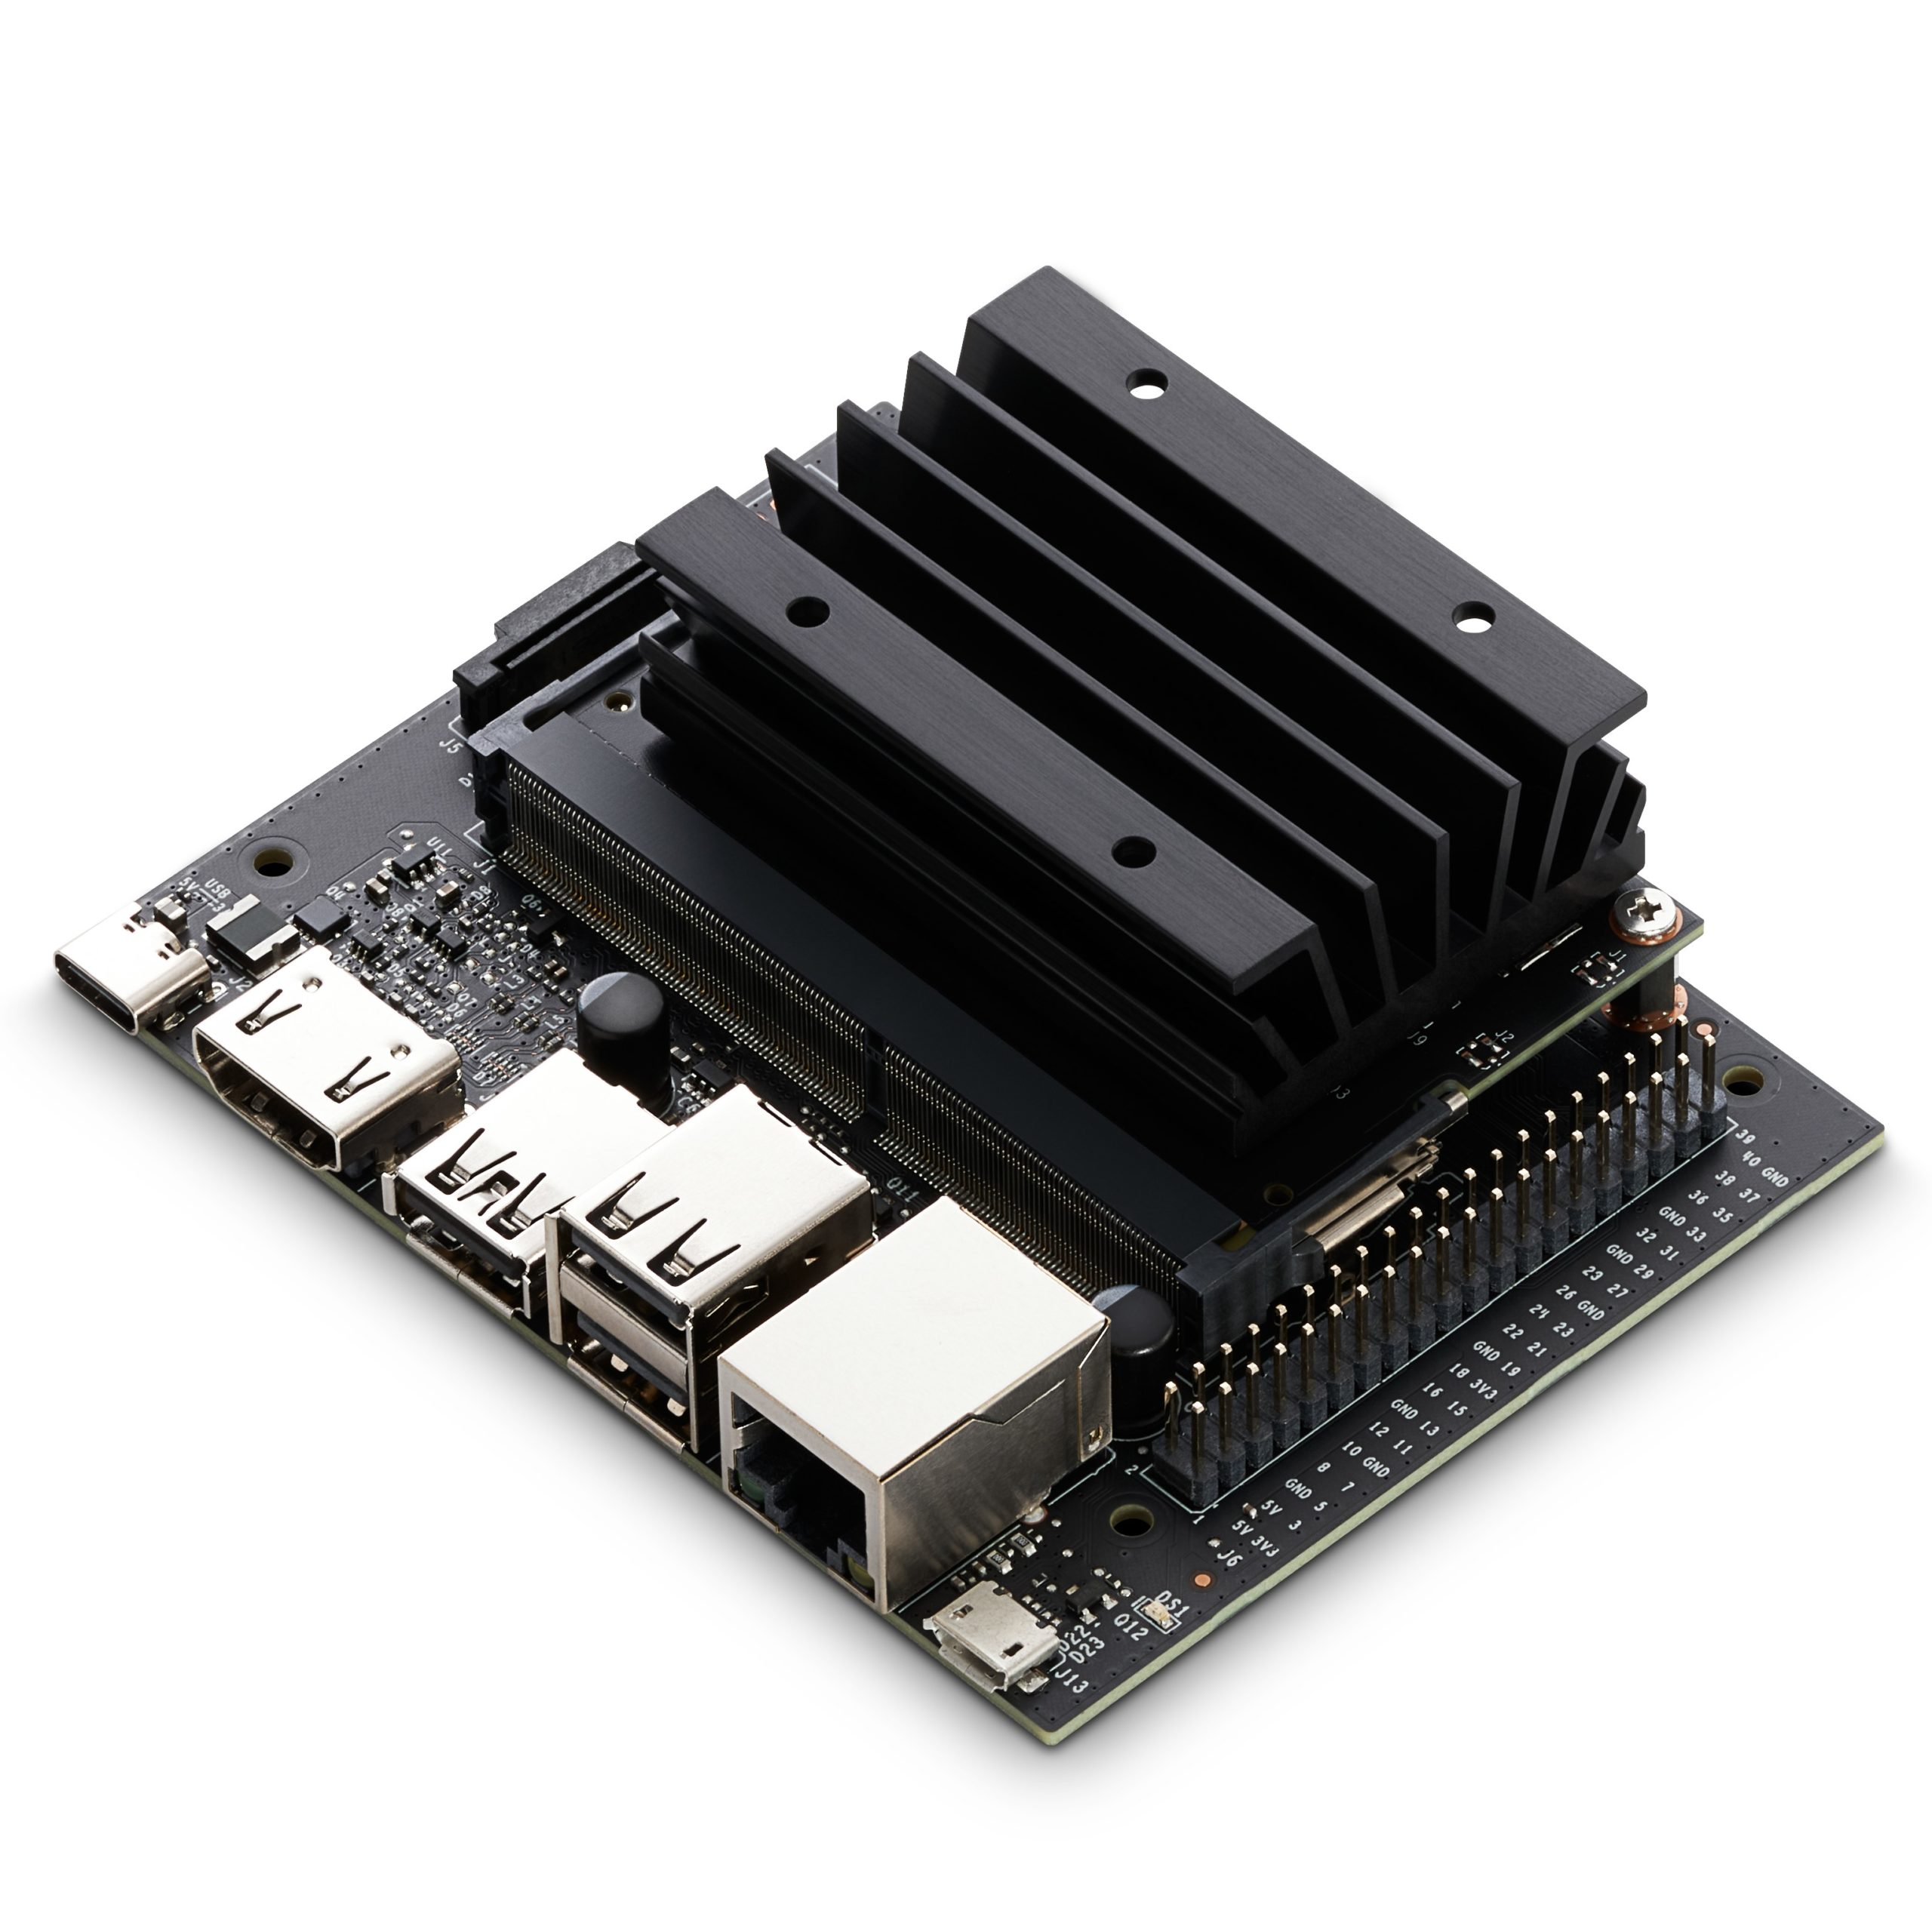
\includegraphics[width=0.5\textwidth]{jetson_nano.jpg}
	\caption{NVIDIA Jetson Nano}\label{fig:jetson-nano}
\end{figure}

\subsection{Cameras}

The selection of appropriate cameras is crucial for the effective operation of the parking management system. The primary requirements for these cameras include weather resistance to withstand heavy rain, the ability to transmit live video feeds to a central computer, and infrared detection capabilities for low-light conditions such as indoor garage parking or nighttime operations. Additionally, the cameras need to be capable of capturing high-quality images to facilitate accurate car detection and license plate identification.

To meet these requirements, several camera models were evaluated. Table \ref{tab:camera_comparison} presents a comparison of the considered options:

\begin{table}
	\begin{tabular}{|l|c|c|c|c|}
		\hline
		\textbf{Specification} & \textbf{Reolink RLC-811A} & \textbf{Lorex Fusion 2K} & \textbf{Eufy Cam S350} & \textbf{Arlo Ultra 2} \\
		\hline
		Resolution             & 4K (8MP)                  & 2K (4MP)                 & 4K (8MP)               & 4K (8MP)              \\
		\hline
		Waterproof             & IP66                      & IP66                     & Indoor only            & IP65                  \\
		\hline
		Infrared               & Yes                       & Yes                      & Yes                    & Yes                   \\
		\hline
		PoE                    & Yes                       & Yes                      & No                     & No                    \\
		\hline
		Price (\euro)          & 166                       & 300                      & 130                    & 399                   \\
		\hline
	\end{tabular}
	\caption{Comparison of Camera Options}\label{tab:camera_comparison}
\end{table}

After careful consideration, the Reolink RLC-811A, see \cref{fig:camera}, was selected as the optimal choice for this project. This camera offers 4K resolution, providing exceptional image clarity for accurate vehicle and license plate detection. Its IP66 weather resistance rating ensures durability in various outdoor conditions, including heavy rain. The camera's built-in infrared capabilities are sufficient for basic low-light operation and can be supplemented with additional infrared lighting when needed.

One of the key advantages of the Reolink RLC-811A is its support for Power over Ethernet (PoE). This feature allows for both power supply and data transmission through a single Ethernet cable, significantly simplifying installation and reducing wiring complexity. The camera's competitive price point of €166 also makes it an attractive option for large-scale deployments across multiple parking facilities.

While the Lorex Fusion 2K offers similar weather resistance and PoE capabilities, its lower 2K resolution may not provide the same level of detail required for accurate license plate recognition. However, it could be a viable alternative if budget constraints become more pressing, as it offers a good balance of features at a mid-range price point.

The Eufy Cam S350, despite its high 4K resolution and lower price, is not suitable for this project due to its lack of weather resistance and PoE capabilities. It is designed for indoor use only, which limits its application in outdoor parking environments.

The Arlo Ultra 2, while offering high-resolution 4K imaging and good weather resistance (IP65), lacks PoE support and comes at a significantly higher price point. Its wireless design, while potentially offering more flexible installation options, may not be ideal for a permanent, large-scale parking management system where consistent power and data connectivity are crucial.

\begin{figure}
	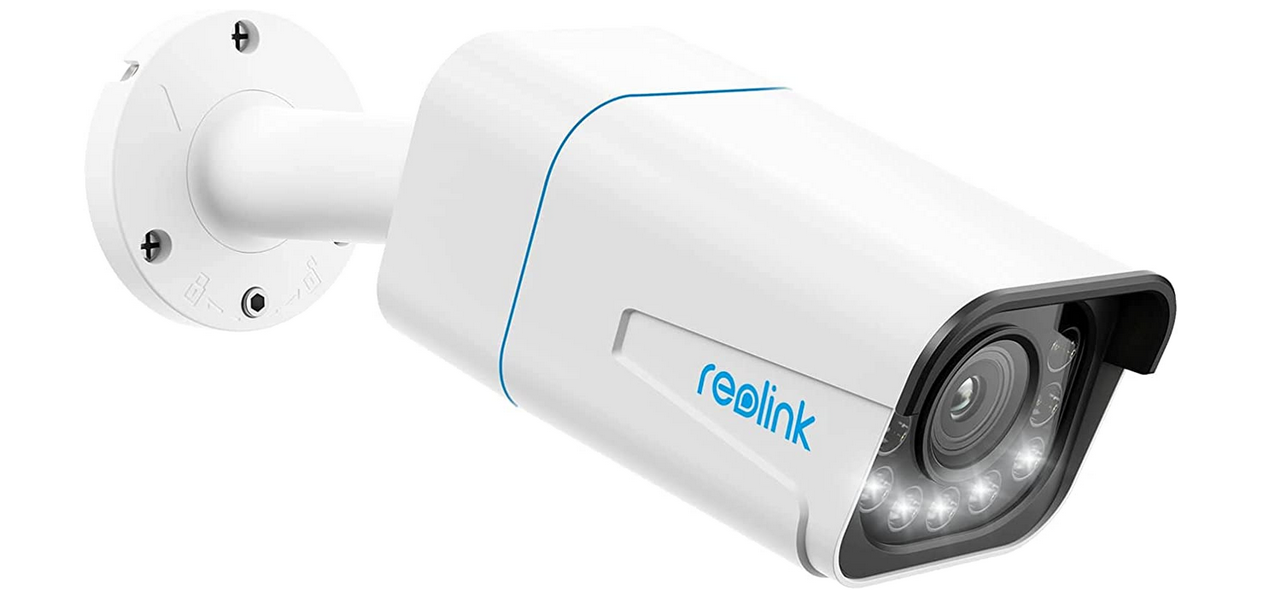
\includegraphics[width=0.5\textwidth]{camera.png}
	\caption{Reolink RLC-811A Camera}\label{fig:camera}
\end{figure}

\subsection{Internet Connectivity}

To provide connectivity from the on-board computer to the server, a networking connection needed to be established. As this deployment must be self-sufficient and not depend on the infrastructure of each community, a router with 4G connection is deployed. For this case, a simple 4G router was used, the TP-Link AC1200. This router offers 4G+ Cat6 connectivity and AC1200 wireless dual-band gigabit capabilities, making it suitable for providing reliable internet access for the parking management system. Moreover, this router has a built-in switch to be able to connect the cameras with the terminal.

\subsection{Server}

The server is the point of contact to connect users with the different communities, facilitating user authentication and enabling connections to specific community resources. It is built on a scalable architecture deployed in AWS (Amazon Web Services), chosen for its rapid time-to-market capabilities and inherent scalability.

AWS provides a cloud-based solution that allows the system to efficiently manage varying loads and adapt to user demand, which is essential for a parking management system that may experience fluctuating traffic patterns. This flexibility ensures that the system can scale up or down seamlessly, accommodating an increasing number of users and devices without compromising performance.

Moreover, AWS offers robust testing environments that allow developers to validate system functionalities before full deployment. This capability is crucial for ensuring reliability and performance under real-world conditions, as it enables iterative testing and refinement of the system components. By leveraging AWS's extensive infrastructure, the project can ensure high availability and resilience, minimizing downtime and enhancing user experience.

In summary, the choice of AWS not only supports the immediate needs of scalability and rapid deployment but also provides a solid foundation for ongoing testing and development, essential for maintaining an effective and responsive parking management solution.



\chapter{Implementation}\label{ch:implementation}

Given the requirements and the design in the previous chapters, refer to \cref{ch:requirements} and \cref{ch:design}, the project is implemented following the V-model established in \cref{ch:methodology_approach}. This chapter describes the implementation of the system, from the architecture to the deployment of the system.

\section{General Architecture}

The architecture, as seen in \cref{fig:architecture}, is composed of two main parts, the server and the communities. The server is in charge displaying the information to the users and the managers and handling the connection between the different communities. The communities are in charge of the detection of the vehicles, the opening of the gates, and the administration of the community (data storage, backup, etc).

\begin{figure}
	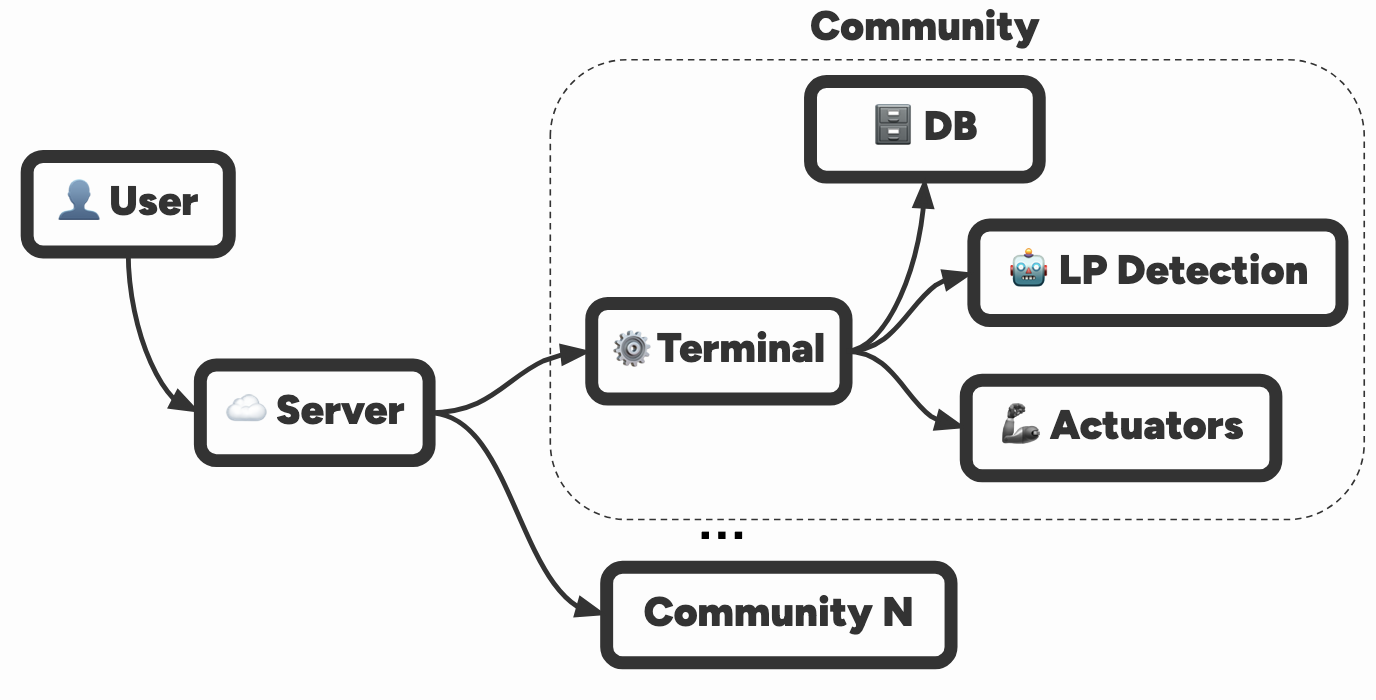
\includegraphics{architecture.png}
	\caption{General Architecture of the system}\label{fig:architecture}
\end{figure}

It is worth noting that the system is design to be scalable and robust, so the system is design to be able to be deployed in different communities and be able to handle the different data and users. That is why in \cref{fig:architecture} multiple communities can be seen.

\section{Community}

The community is a collection of the systems to provide the ability to open the gates, detect the vehicles, and store the data for a single building or community. A community is usually composed of three main subsystems, the licence plate detection system, the terminal server, and the actuators. Moreover, the community is connected to the internet to be able to connect to the server and perform other actions such as updates, remote administration, etc.

\subsection{Licence Plate Detection System}

The first component of the sytems is the detection of the licence plates. The detection of the licence plates is done by a deep learning algorithm that detects the licence plates in the images. The detection algorithm is based on YOLO \autocite{yolov8_ultralytics} and is implemented in the terminal. The detection algorithm is in charge of detecting the licence plates in the images and sending the data to the database.

The implementation of the algorithm is out of the scope of this project, and it is based on the Dual Licence Plate Recognition system \autocite{RAMAJOBALLESTER2024104608}. The system is composed of two main steps, the detection of the licence plate and the detection of the characters of the licence plate. Some examples can be seen in \cref{fig:licence_plate_detection}.

\begin{figure}
	\begin{subfigure}{0.95\textwidth}
		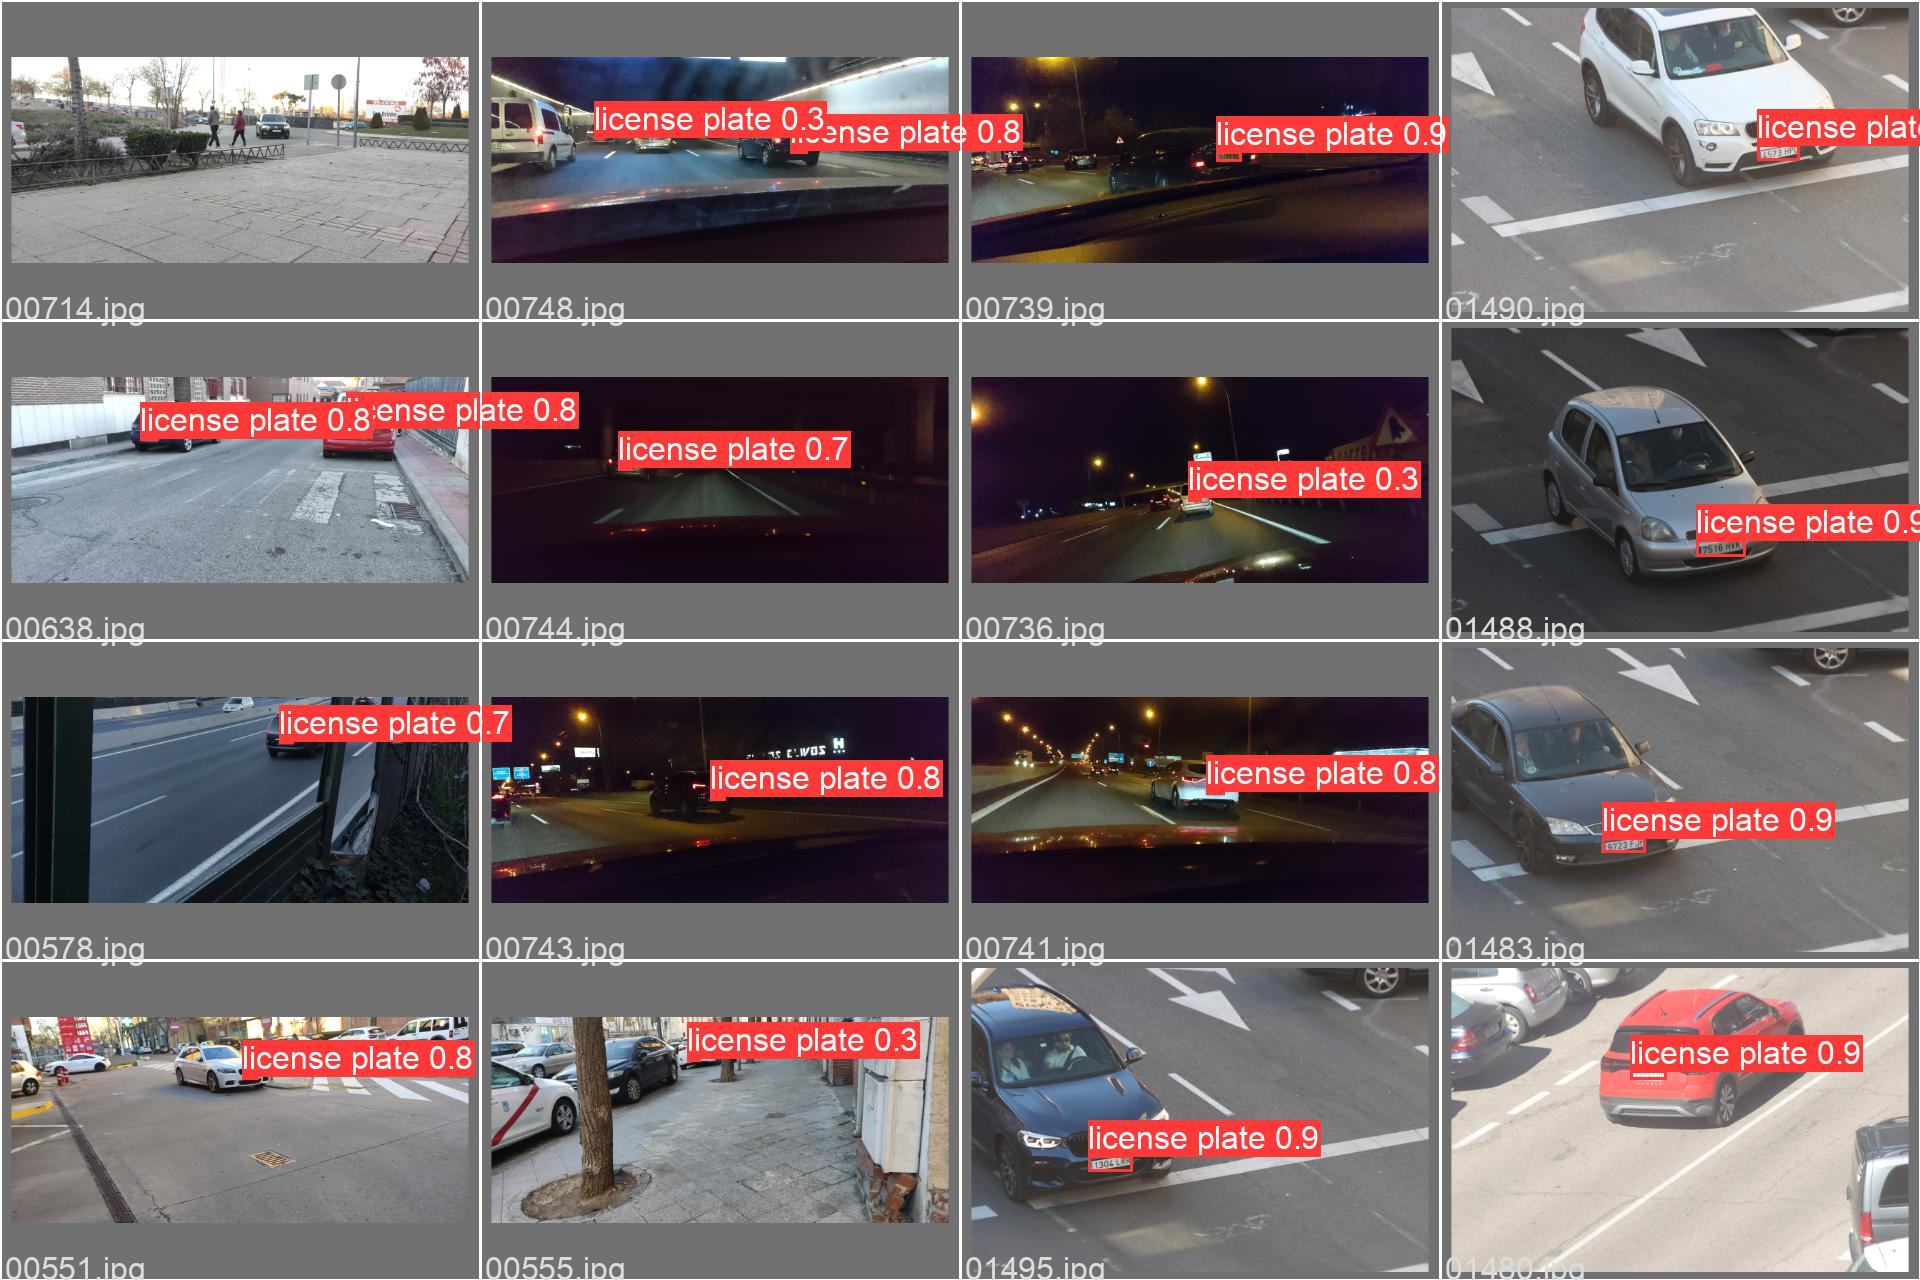
\includegraphics{licence_plate_recognition.jpg}
		\caption{Testing of the Licence Plate Detection System. \autocite{RAMAJOBALLESTER2024104608}}
	\end{subfigure}
	\br
	\begin{subfigure}{0.95\textwidth}
		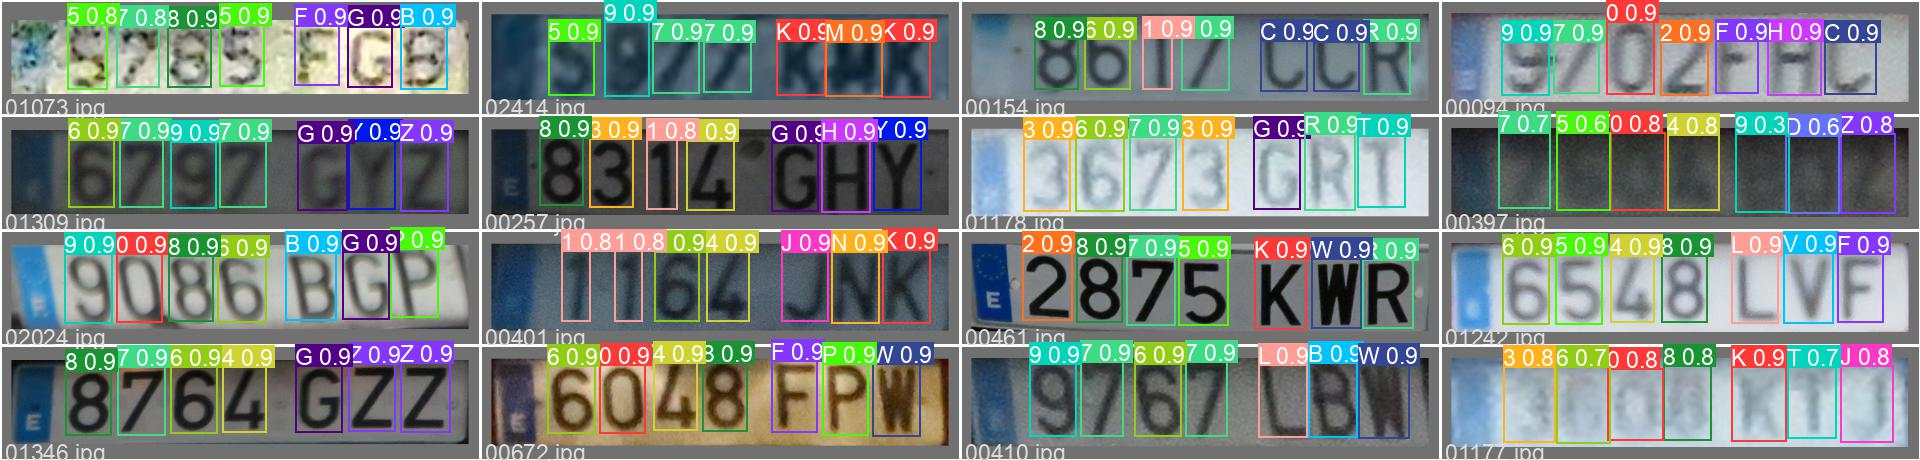
\includegraphics{ocr_licence_plate.jpg}
		\caption{Testing of the OCR character detection of the Licence Plate Detection System. \autocite{RAMAJOBALLESTER2024104608}}
	\end{subfigure}

	\caption{Licence Plate Detection alghorithms. \autocite{RAMAJOBALLESTER2024104608}}\label{fig:licence_plate_detection}
\end{figure}

\subsection{Terminal Server}

To provide the main functionality of the system, a terminal server is used. The terminal server is in charge of the communication between the different subsystems of the community and the server. The terminal server is in charge of communicating with the server, the actuators, the detection algorithm, the data storage, the backup of the data, and the user administration.

For reference, the terminal server is designed ot be run on any Linux system, and the implementation is based on the ExpressJS framework. This makes the terminal server easy to deploy and maintain. Moreover, the terminal server is design to be able to be updated remotely and be able to be connected to the internet.

For the communication between the different subsystems, the terminal server uses a RestAPI methodology. This allows the different subsystems to communicate with the terminal server and perform the different actions.

\subsubsection{Database}

Different architecture approaches were considered for the database, such as SQL or NoSQL databases, local or cloud databases. For this project, a local SQL database based on SQLite is used. The main reason behind this decision was the requirement of having the data inside the community for data privacy and security reasons. The SQL architecture is used as it provides a robust and reliable way to store the data and be able to perform the different actions required such as filtering, searching, and more. The database architecture can be seen in \cref{fig:database_architecture}.

\begin{figure}
	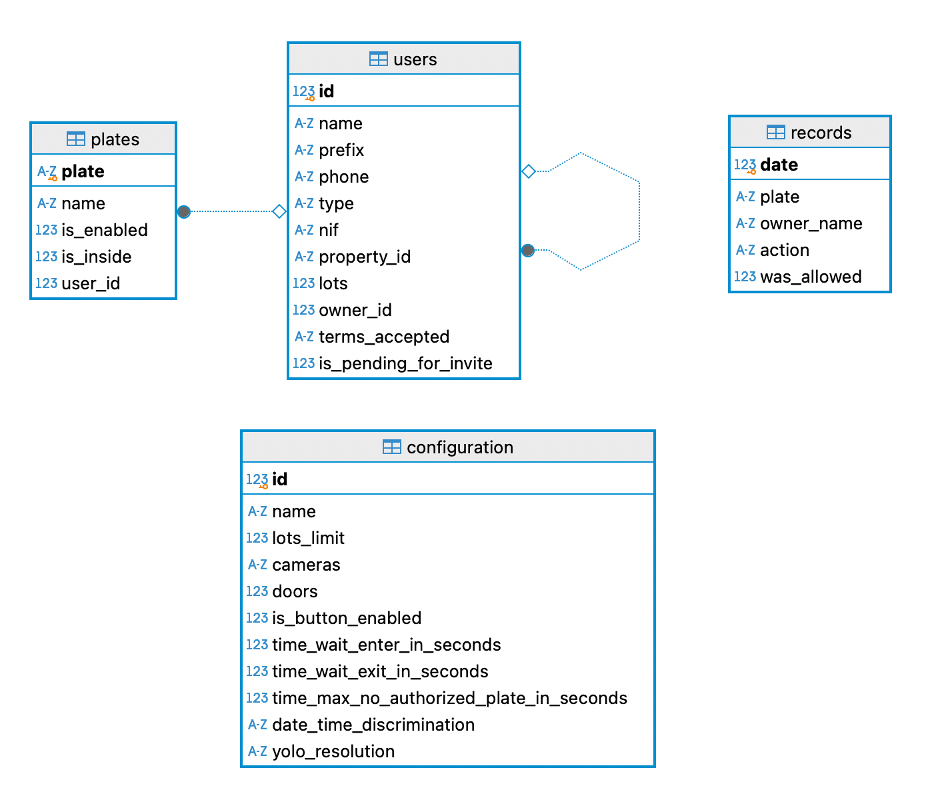
\includegraphics{database_architecture.png}
	\caption{Database Architecture}\label{fig:database_architecture}
\end{figure}

The database is divided into four main tables to store the different types of data.

The first table is the \texttt{users} table. This table is in charge of storing the information of the users of the system. The table is composed of the following fields:

\begin{itemize}
	\item \texttt{id}: The unique identifier of the user which is a autoincrement numeric field.
	\item \texttt{name}: The name of the user to identify it.
	\item \texttt{prefix}: The prefix of the phone used by the user, as the users come from different countries.
	\item \texttt{phone}: The phone number of the user.
	\item \texttt{type}: The type of the user, which can be either an administator, an owner of a property, or a visitor.
	\item \texttt{nif}: The NIF of the user, which is used to identify the user for regulatory and security reasons.
	\item \texttt{property\_id}: The identifier of the property of the user.
	\item \texttt{lots}: The number of parking spaces that the user has.
	\item \texttt{owner\_id}: Id of the owner of the property if the user is a visitor.
	\item \texttt{terms\_accepted}: A boolean field to check if the user has accepted the terms and conditions of the system.
	\item \texttt{is\_pending\_for\_invite}: A boolean field to check if the user is pending for an invitation to the system.
\end{itemize}

The primary key of the table is the \texttt{id} field. And a foreign key is used to connect the \texttt{owner\_id} field to the \texttt{id} field between an owner and a visitor. Moreover, different check are performed to ensure the data integrity and the security of the data, for example, the \texttt{phone} field is checked to be a valid phone number and unique.

Secondly, the \texttt{plates} table is used to store the information of the licence plates registed in the system. The table is composed of the following fields:

\begin{itemize}
	\item \texttt{plate}: Alphanumeric field to store the licence plate, the length is variable to adapt to different countries.
	\item \texttt{name}: Identifier of the licence plate for easy identification.
	\item \texttt{is\_enabled}: Boolean field to check if the licence plate is enabled or disabled, that is, if it is allowed to enter the community.
	\item \texttt{is\_inside}: Boolean field to check if the licence plate is inside the community in order to have a control of the vehicles inside the community.
	\item \texttt{user\_id}: The identifier of the user that owns the licence plate.
\end{itemize}

The primery key of the table is the \texttt{plate} field. A foreign key is used to connect the \texttt{user\_id} field to the \texttt{id} field of the \texttt{users} table. Moreover, the \texttt{plate} field is checked to be unique and the \texttt{user\_id} field is checked to be a valid user.

For the configuration of the community, the \texttt{configuration} table is used. The table is composed of the following fields:

\begin{itemize}
	\item \texttt{id}: The unique identifier of the configuration. As there is only one configuration, the field is a constant and set to 1 by default.
	\item \texttt{name}: The identifier name of the community.
	\item \texttt{lots\_limit}: The maximum number of parking spaces in the community.
	\item \texttt{cameras}: The configuration of the cameras in the community. It is used to match the specific cameras with the specific actuators of the community.
	\item \texttt{doors}: The number of garage doors in the community as multiple doors can be used for different points of the community.
	\item \texttt{is\_button\_enabled}: Boolean field to check if the button to open the door is enabled to be able to open the door manually.
	\item \texttt{time\_wait\_enter\_in\_seconds}: Timeout to wait for a vehicle to enter the community.
	\item \texttt{time\_wait\_exit\_in\_seconds}: Timeout to wait for a vehicle to exit the community.
	\item \texttt{time\_max\_no\_authorized\_plate\_in\_seconds}: Timeout to wait for a vehicle to enter the community if the licence plate is not authorized.
	\item \texttt{date\_time\_discrimination}: Variable to check if the system is using the date and time to discriminate the vehicles.
	\item \texttt{yolo\_resolution}: Configuration for the Licence Plate Detection System.
\end{itemize}

The primary key is the \texttt{id} field and it is set to 1 in order to only have one configuration. This information is kept in the database to centralized everything and make it easier to backup the data. A separate file can be used for the configuration, but it is stored in the database for security reasons.

Finally, the \texttt{records} table is used to store the logs of the system, that is all the different interactions with the different subsystems, such as the licence plates detected, the users that enter the community, the users that exit the community, etc. The table is composed of the following fields:

\begin{itemize}
	\item \texttt{date}: The timestamp of the record.
	\item \texttt{plate}: The licence plate of the vehicle that is detected.
	\item \texttt{owner\_name}: The name of the owner of the vehicle that is detected to have a better control of access flow.
	\item \texttt{action}: The action performed, that is, if the vehicle is entering or exiting the community.
	\item \texttt{was\_allowed}: Boolean field to check if the vehicle was allowed to enter the community.
\end{itemize}

The primary key of the table is the \texttt{date} field, this is done to restrict multiple different records for a sigle timestamp. Moreover, the \texttt{date} field is set to use the ISO 8601 format to have a standard format for the date and time.

As the terminal is situated in the community, unauthorized access to the database is a concern. To keep the database secured from unauthorized access, the database is encrypted using the SQLCipher library. This library is used to encrypt the database and ensure that the data is secure and only accessible by the system. Keeping the database encrypted ensures that the data is secure and only accessible by the system.

\subsubsection{Application Programming Interface}

As stated previously, in order to communicate with the different subsystems, a RestAPI is used. The RestAPI is used to perform the different actions such as opening the door, detecting the licence plates, storing the data, etc. The RestAPI is built using the ExpressJS framework, as it is easy to use and maintain. For this different endpoints are used to perform the different actions such as user administration, licence plate detection, door opening, etc. In order to perform the authenicaton of the users, JWT tokens are used to ensure that the request is performed by the right user. The authenicaton process is later outlined in \cref{sec:authentication}.

\subsubsection{Actuators}

To interact with the various subsystems of the communities, particularly for controlling access points like garage doors, the system employs a custom Relay Expansion Board designed for the NVIDIA Jetson Nano. This board serves as the interface between the digital control signals from the terminal server and the physical actuators. The choice of this solution came after studying different door opening systems, all of which required a signal to be pulled down to ground to trigger the mechanism.

The control of doors is achieved through relays, which act as electrically operated switches. To enable both automated and on-demand operation of the doors, a small server is set up within the terminal. This server listens for requests to open the door, which can come from either the license plate recognition system or authorized user commands.

When a valid request is received by the server, it processes the command and sends an appropriate signal to the Relay Expansion Board. The board then activates the corresponding relay, which in turn triggers the door mechanism to open. This setup allows for seamless integration of the automated license plate recognition system with manual override capabilities, ensuring flexibility and reliability in access control.

The use of relays provides several advantages. It offers electrical isolation between the control circuitry and the door mechanisms, allows for the control of high-voltage or high-current devices with low-voltage signals, and provides flexibility to adapt to various types of door actuators used in different communities.

This actuator subsystem is crucial in translating the software-based decisions of the parking management system into physical actions, effectively bridging the digital and physical aspects of the solution. The system's ability to open doors based on both automated detection and manual requests ensures a versatile and user-friendly operation, catering to different scenarios and user needs within the parking management ecosystem.

\subsubsection{Other subsystems}

The system incorporates several additional components that work together to ensure reliable operation and data integrity. The surveillance infrastructure utilizes a network of cameras strategically positioned throughout the community, particularly at entry and exit points. Each camera captures video feeds and transmits them to the terminal for processing using the Real-Time Streaming Protocol (RTSP). The cameras connect to the network infrastructure via Ethernet cables, ensuring stable and high-quality video transmission.

Network connectivity is managed through a dedicated 4G router equipped with an integrated switch. This router, specifically the TP-Link AC1200 model, serves two critical functions: it facilitates communication between the cameras and the terminal, and provides internet connectivity for the entire system. The choice of a 4G router ensures that the system remains independent of the community's existing infrastructure while maintaining reliable connectivity. The integrated switch allows for efficient connection of multiple cameras and the terminal, simplifying the network topology and reducing potential points of failure.

To ensure data integrity and business continuity, the system implements a comprehensive backup strategy. The database, which contains critical operational data including user information and access logs, is automatically backed up daily to Amazon S3 \autocite{AmazonS3}. These backups are encrypted both during transmission and storage, protecting sensitive information from unauthorized access. This automated backup system ensures a \gls{rpo} of 24 hours, minimizing potential data loss in the event of system failure or data corruption. The combination of local encrypted storage and cloud-based backups provides a robust solution for data protection and recovery.

\section{Cloud deployment}

To enable the access to the different communities from the user point of view, a web server is deployed in AWS. The main component is a NextJS server that holds the website that the users use to access the system and also the backend functionality to connect to each specific community.

\subsection{Cloud Architecture}

The cloud architecture developed for this project adopts a cost-effective and scalable methodology, leveraging Amazon Web Services (AWS) as the primary cloud provider. As illustrated in \cref{fig:cloud_architecture}, the architecture employs a distributed design that prioritizes reliability and security while maintaining operational efficiency.

\begin{figure}
	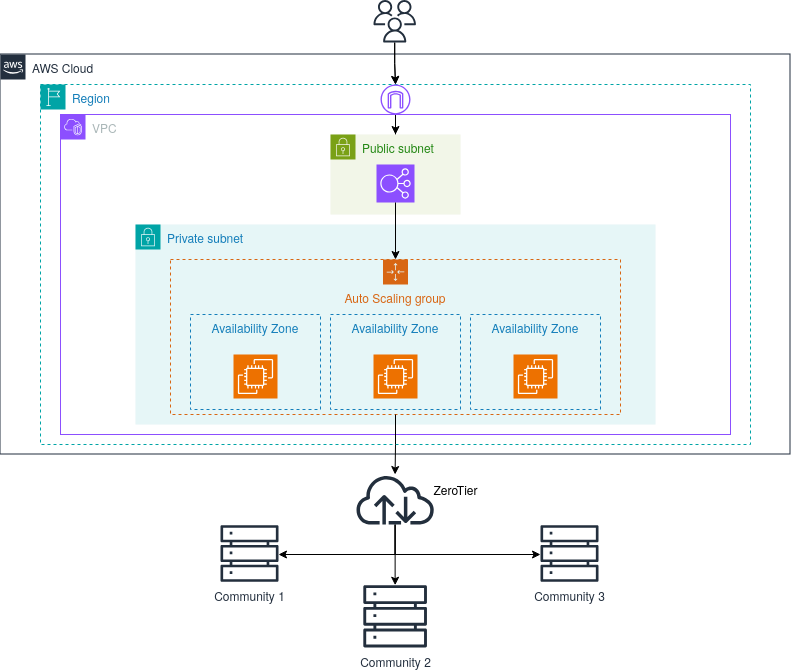
\includegraphics{cloud_architecture.png}
	\caption{AWS Cloud Architecture} \label{fig:cloud_architecture}
\end{figure}

During the development phase, several architectural approaches were evaluated, including serverless computing, container-based solutions, and traditional virtual machine deployments. While serverless and container architectures offered certain advantages in terms of scalability and maintenance, the specific requirements of the networking component, particularly the integration with ZeroTier, necessitated the use of EC2 instances. This decision was primarily driven by ZeroTier's requirement for low-level network access and administrative privileges, which are not readily available in more abstracted deployment models.

The architecture is implemented within AWS's Virtual Private Cloud (VPC), which provides network isolation and security. Public and private subnets are utilized to create a layered security approach, with the public subnet hosting load balancers and other internet-facing components, while the private subnet contains the application servers and sensitive resources. This separation ensures that critical system components remain protected from direct external access.

To ensure high availability and fault tolerance, the EC2 instances are distributed across multiple Availability Zones within the chosen AWS region. An Auto Scaling group manages these instances, automatically adjusting capacity based on demand while maintaining optimal performance and cost efficiency. This approach allows the system to handle varying loads while minimizing operational expenses.

The networking layer is particularly crucial in this architecture, as it must facilitate secure communication between the cloud infrastructure and the distributed community terminals. ZeroTier integration, later explained in \cref{sec:networking}, enables the creation of secure, encrypted tunnels between AWS resources and on-premises community systems, effectively establishing a hybrid cloud environment that maintains both security and performance.

This architectural design successfully balances the requirements for scalability, security, and cost-effectiveness, while providing the necessary infrastructure to support the parking management system's distributed nature. The use of EC2 instances, though more traditional than newer deployment options, proves to be the most suitable choice for meeting the specific networking and security requirements of the system.

\subsection{Website}

The website component of the parking management system is designed with a strong focus on user experience and accessibility across different devices. Built using the React framework \autocite{react}, the website provides a modern, interactive interface that enables users to manage their parking spaces and access system features efficiently. React's component-based architecture facilitates the development of reusable interface elements while ensuring optimal performance through its virtual DOM implementation.

For styling and visual presentation, the website implements TailwindCSS \autocite{tailwindcss}, a utility-first CSS framework that enables rapid development of custom, responsive designs. This approach allows for consistent styling across different screen sizes while maintaining a clean, modern aesthetic that aligns with contemporary web design standards. The combination of React and TailwindCSS creates a robust foundation for building an intuitive user interface that adapts seamlessly to various device sizes and orientations.

An example of the website can be seen in \cref{fig:website_example}. The capabilities of the website are login, register, manage the different users, manage the different parking spaces, and manage the different configurations of the community. Moreover, the different records can be seen by the administrators.

The responsive design implementation ensures that the website functions effectively on both desktop computers and mobile devices, with layouts and interactions optimized for touch interfaces when accessed on smartphones or tablets. This adaptability is crucial for users who need to access the parking management system while on the move, particularly for tasks such as remotely opening garage doors or managing visitor access.

To enhance accessibility and provide a more native-like experience on mobile devices, the website is also implemented as a Progressive Web App (PWA). This implementation allows users to install the website as a standalone application on their Android or iOS devices directly from their respective app stores. The PWA approach combines the best aspects of web and native applications, offering features such as offline functionality, push notifications, and improved performance through local caching mechanisms.

The PWA implementation follows modern web standards and best practices, ensuring compatibility across different mobile platforms while maintaining a consistent user experience. This approach eliminates the need for platform-specific native applications while still providing the convenience and functionality users expect from a mobile app. Users can access features such as real-time parking space monitoring, license plate management, and access control directly from their home screens, making the system more accessible and user-friendly.

Moreover, the website is embeded in Progressive Web Apps in Android and iOS to allow users to download an application through the mobile store of choice and be able to use the website in their phones, \cref{fig:mobile_app}. It is worth noting that the application is a wrapper of the website, but it allows the users to have a more native experience. For the iOS version, the application is not available in the App Store, as the App Store has a more strict policy for the applications and it is currently under review.

\begin{figure}
	\hfill
	\begin{subfigure}{0.45\textwidth}
		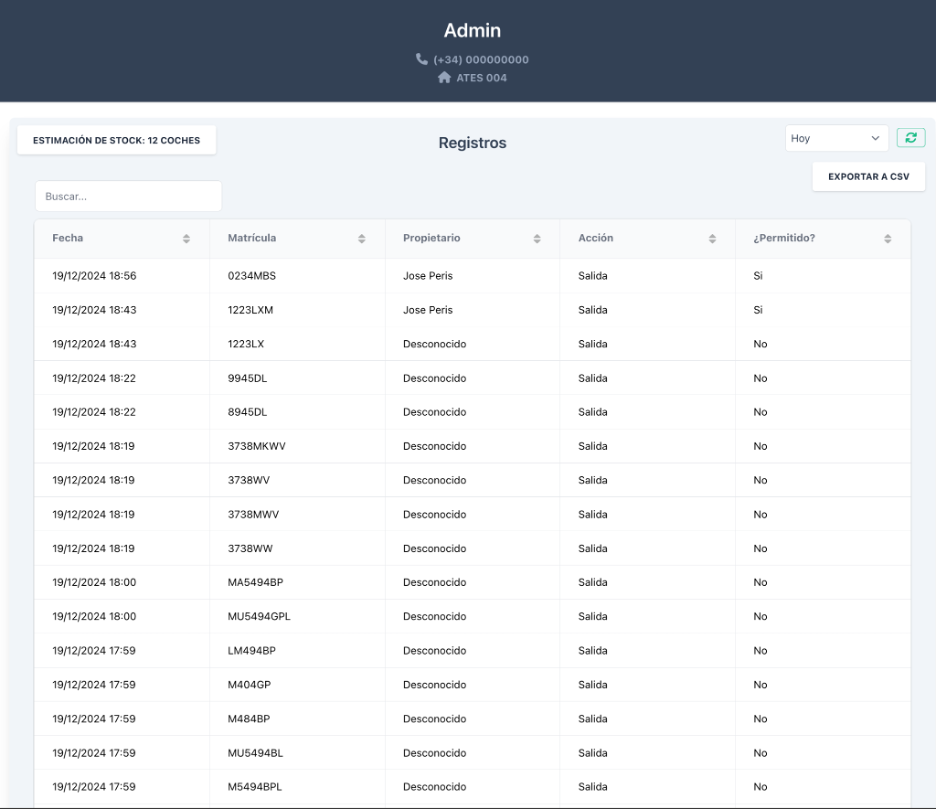
\includegraphics{website_example.png}
		\caption{Website Example.}\label{fig:website_example}
	\end{subfigure}
	\hfill
	\begin{subfigure}{0.45\textwidth}
		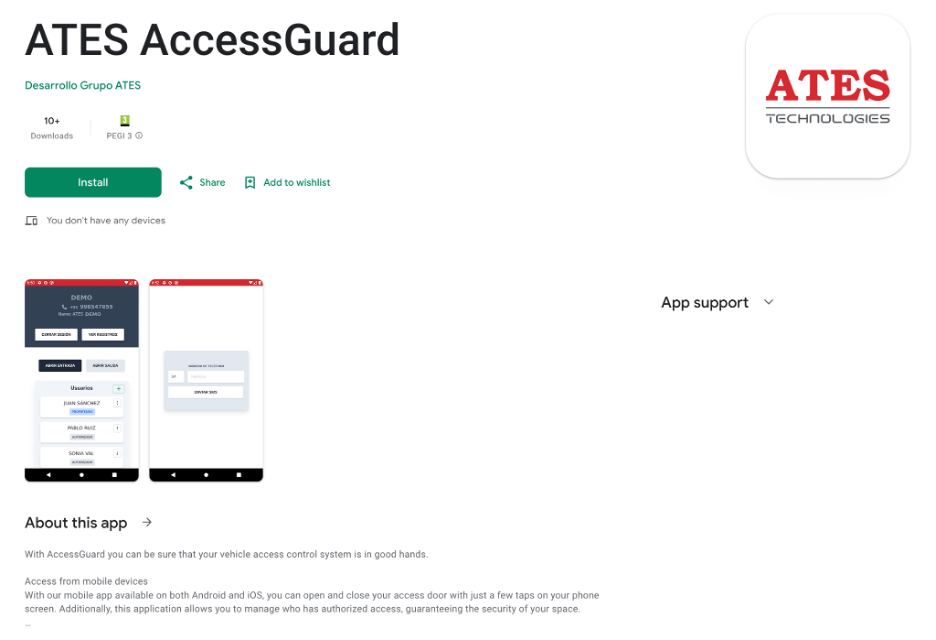
\includegraphics{mobile_app.png}
		\caption{Android Applciation deployed in Google Play Store}\label{fig:mobile_app}
	\end{subfigure}
	\hfill

	\caption{Website design and mobile application.}
\end{figure}

\subsection{Networking}\label{sec:networking}

The interconnection of diverse communities with the web server in a decentralized and user-friendly manner is achieved through the implementation of ZeroTier \autocite{zerotier2025}. This innovative Wide LAN technology facilitates the connection of various devices across the internet by establishing secure VPN tunnels. ZeroTier proves to be an excellent solution for linking different communities to the web server, enabling a range of functionalities such as door access control and license plate recognition.

One of the primary motivations for utilizing EC2 instances in the cloud deployment was the seamless integration of ZeroTier. This approach eliminates the need for proxies or other intermediary measures, streamlining the overall system architecture. The direct installation of ZeroTier alongside the server on EC2 instances ensures a robust and efficient networking solution.

Furthermore, ZeroTier offers the invaluable capability of remote control access. This feature significantly enhances the ability to debug and troubleshoot issues within different communities without the necessity of on-site presence. Technicians and administrators can remotely access the system, diagnose problems, and implement solutions, greatly reducing response times and improving overall system maintenance.

The decentralized nature of ZeroTier aligns well with the project's goals of creating a flexible and scalable network infrastructure. As new communities are added to the system, they can be easily integrated into the existing network topology without major reconfiguration. This scalability ensures that the system can grow organically as more communities adopt the technology.

Security is another crucial aspect addressed by the ZeroTier implementation. The VPN tunnels created by ZeroTier provide encrypted communication channels, safeguarding sensitive data transmitted between the communities and the central web server. This encryption is particularly important when dealing with access control systems and personal information associated with license plate recognition.

In summary, the adoption of ZeroTier as the networking solution for this project offers a powerful combination of ease of use, scalability, remote management capabilities, and enhanced security. These features collectively contribute to a robust and efficient system that can reliably serve multiple communities while remaining adaptable to future growth and technological advancements.


\subsection{User Authentication}\label{sec:authentication}

The authentication system for this project implements a phone-based SMS verification approach, prioritizing both security and user experience. This decision was driven by the requirement to create a simple yet secure authentication process that would be easily accessible to all users, regardless of their technical expertise. Traditional password-based systems often lead to security vulnerabilities due to weak password choices or password reuse, making SMS-based authentication an attractive alternative.

Firebase Authentication was selected as the authentication provider for this implementation, offering a robust and scalable solution for handling SMS-based user verification. This service manages the entire SMS delivery and verification process, including phone number validation, SMS dispatch, and code verification. Firebase's global infrastructure ensures reliable message delivery across different cellular networks and geographical regions, which is crucial for a system deployed across multiple communities.

The authentication flow begins when a user attempts to access the system. They are prompted to enter their phone number, which is then validated for format correctness. Firebase Authentication sends a one-time verification code via SMS to the provided number. This temporary code must be entered by the user within a specified timeframe to complete the authentication process. Upon successful verification, Firebase generates a JSON Web Token (JWT) that serves as the user's authentication credential for subsequent interactions with the system, see \cref{fig:firebase} for reference.

These JWT tokens play a crucial role in maintaining security across the distributed architecture. When a user makes requests to either the cloud server or the terminal servers in specific communities, the JWT token is included in the request headers. The receiving systems verify the token's authenticity using Firebase's public keys, ensuring that only requests from properly authenticated users are processed. The tokens contain encoded information about the user's permissions and access levels, allowing the system to enforce appropriate access controls without requiring additional database queries.

To enhance security further, the tokens are configured with appropriate expiration times, requiring periodic re-authentication. This helps mitigate the risk of token theft or unauthorized access. Additionally, the system maintains a blacklist of revoked tokens to handle cases where immediate access termination is required, such as when a user's privileges are revoked or suspicious activity is detected.

The entire authentication process is integrated seamlessly into both the web interface and mobile applications, providing a consistent user experience across all platforms. Error handling mechanisms are implemented to manage various edge cases, such as failed SMS delivery, network connectivity issues, or invalid verification codes, ensuring that users receive clear feedback and guidance throughout the authentication process.

\begin{figure}
	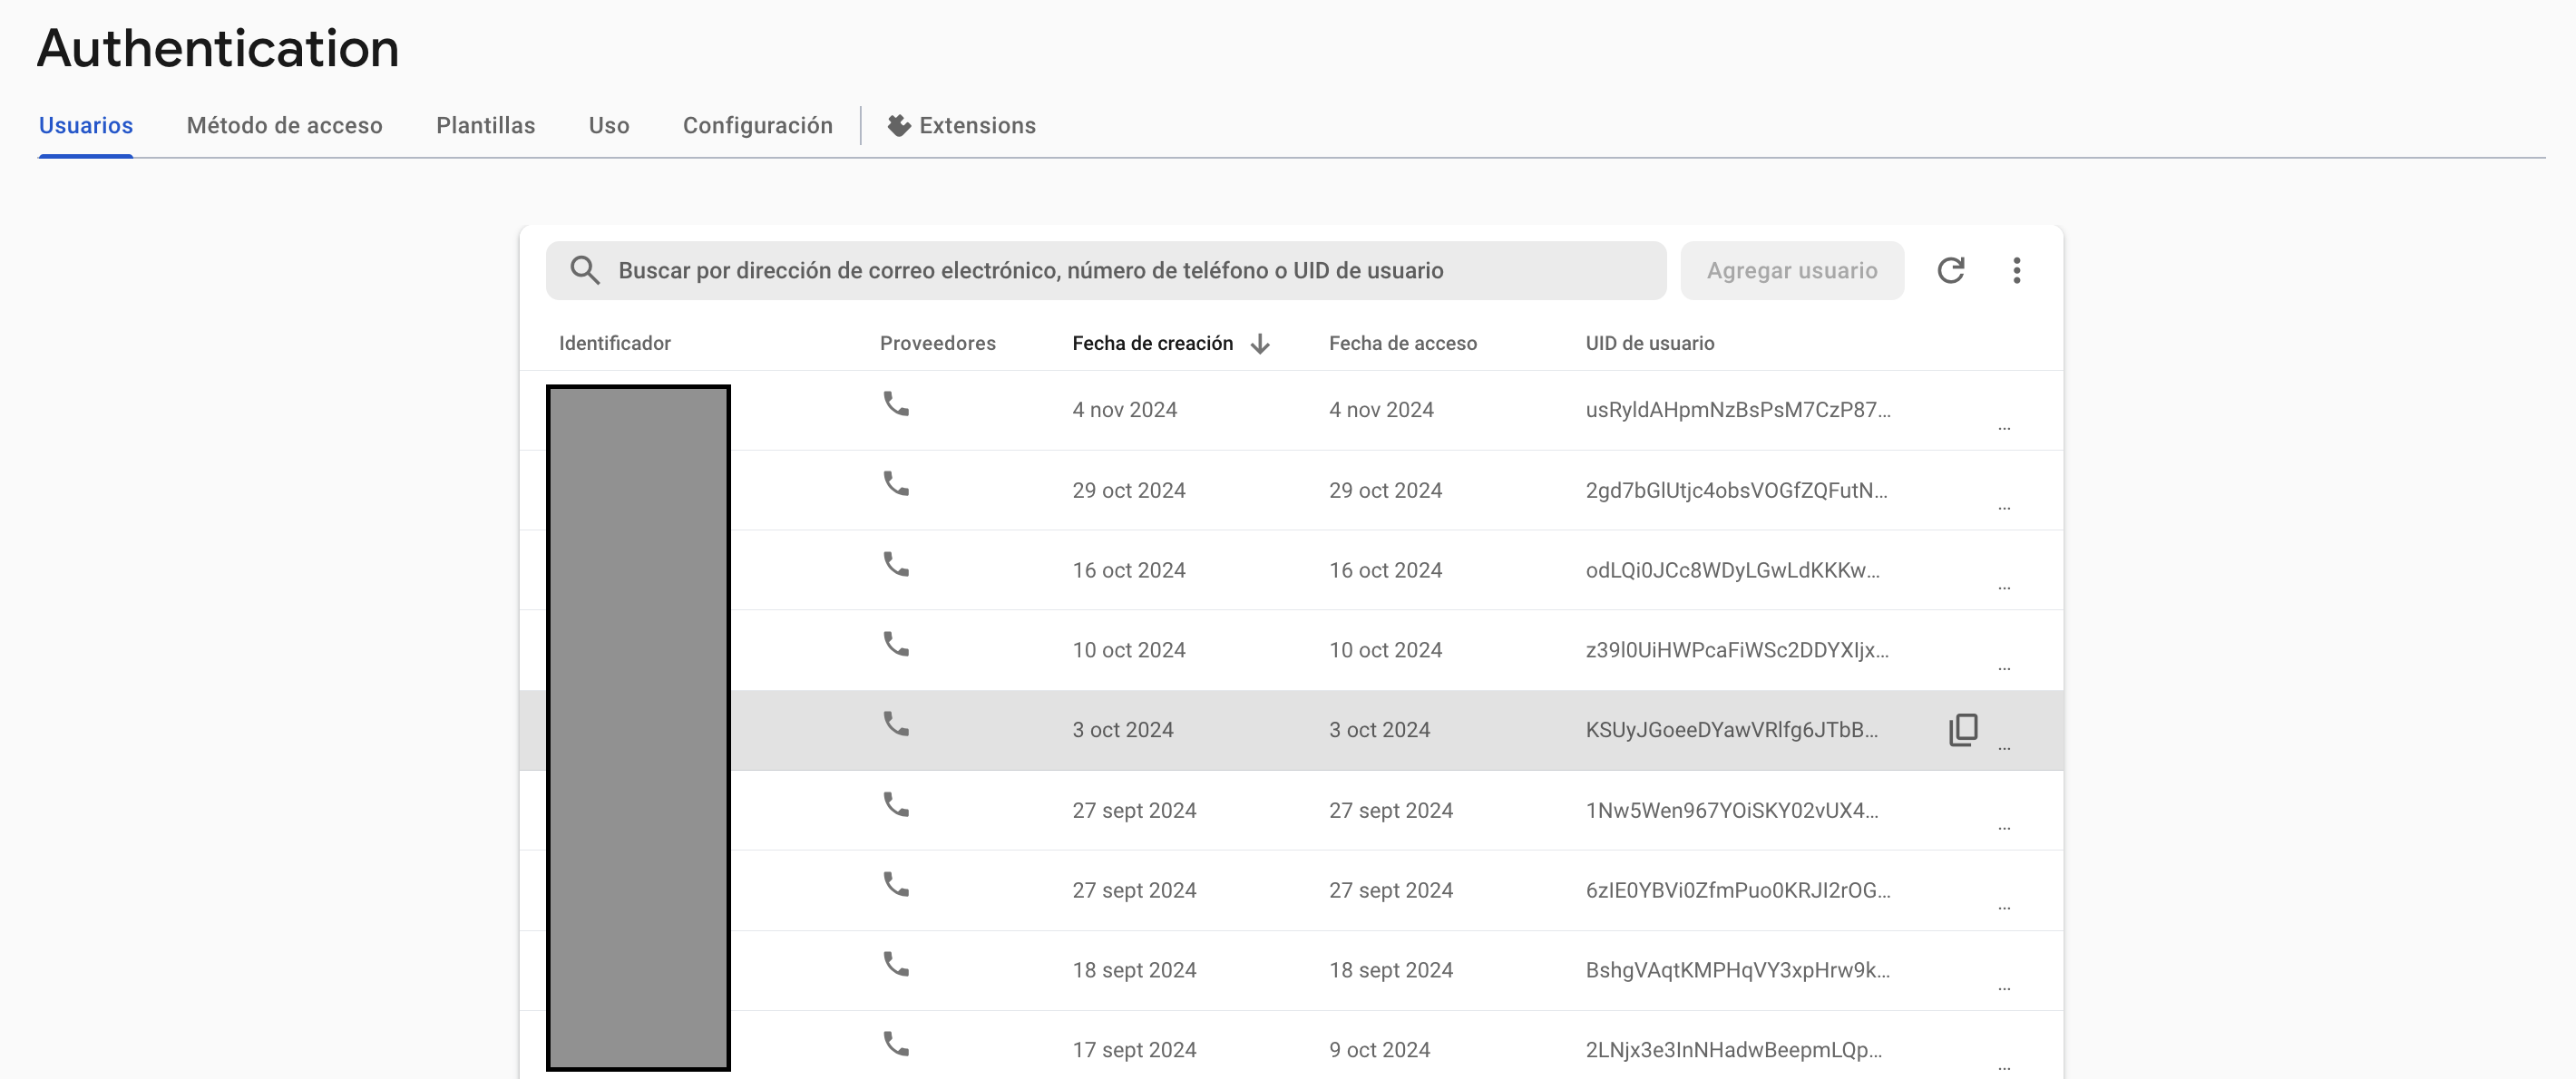
\includegraphics{firebase.png}
	\caption{Firebase Authentication Users example}\label{fig:firebase}
\end{figure}

\section{Deployment}

The deployment process for this distributed parking management system encompasses multiple components, including terminal servers in communities and cloud-based web servers. A standardized approach leveraging modern continuous integration and deployment practices ensures consistent and reliable software updates across all system components. The foundation of this deployment strategy relies on JavaScript frameworks, with applications built and managed through the NPM package manager. To automate the build and release process, a sophisticated GitHub Action pipeline triggers whenever a new release is created in the Git repository. An example can be seen in \cref{fig:github_actions} where web server can be built for the \texttt{0.3.2} version.

\begin{figure}
	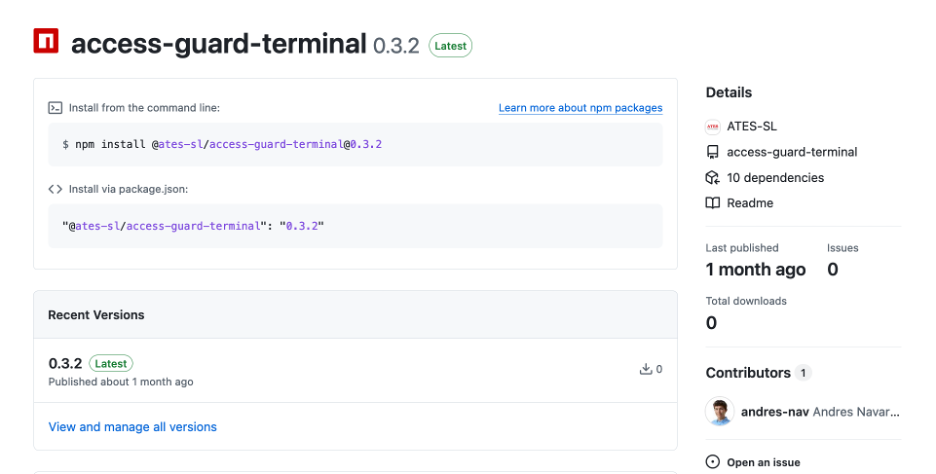
\includegraphics[width=0.7\textwidth]{github_actions.png}
	\caption{Example of the GitHub Actions Pipeline}\label{fig:github_actions}
\end{figure}

The deployment pipeline is designed to handle the complexities of distributing software across various environments while maintaining system integrity and security. When a new version is tagged in the Git repository, the GitHub Actions workflow automatically initiates the build process, creating NPM packages with all necessary dependencies. These packages are then stored in GitHub Packages, providing a centralized and secure location for distribution to both community terminals and cloud servers.

\subsection{Terminal Deployment}

The deployment of community terminals requires special consideration due to their distributed nature and the critical importance of maintaining data integrity. Terminal software updates are managed through automated processes, but database migrations present unique challenges. Currently, database migrations are handled manually to ensure data integrity and prevent potential issues that could arise from automated migration processes. This conservative approach reflects the critical nature of the parking management data and the need to maintain system reliability.

While this manual database migration process is functional, it represents an area identified for future improvement. Work is ongoing to design a robust automated migration system that can maintain data integrity while reducing the operational overhead of manual interventions. This enhancement will need to carefully balance automation with data safety, ensuring that no critical information is lost or corrupted during updates.

To ensure the continuous operation of services on the terminals, systemd services have been implemented. These services are configured to start automatically when the system boots, ensuring that all necessary components of the parking management system are up and running without manual intervention. This approach enhances the reliability and uptime of the terminal systems.

A backup system has been integrated to safeguard critical data. This system automatically uploads the terminal's database to Amazon S3, a secure cloud storage service. Regular backups ensure that data can be recovered in case of hardware failure or other unforeseen issues, minimizing the risk of data loss.

The integration with ZeroTier plays a crucial role in networking the terminals. ZeroTier creates a secure, virtual network that connects all terminals to the central server, regardless of their physical location. This setup allows for easy management and communication between the terminals and the central system, while maintaining a high level of security.

To facilitate these processes, custom scripts have been developed. These scripts automate various tasks such as initiating backups, managing ZeroTier connections, and handling routine maintenance tasks. The use of custom scripts allows for a high degree of flexibility and customization, ensuring that the specific needs of the parking management system are met efficiently.

These enhancements to the terminal deployment process contribute to a more robust, secure, and manageable system. They address key aspects of system reliability, data protection, and network connectivity, which are essential for the effective operation of a distributed parking management solution.

\subsection{Server Deployment}

The cloud infrastructure deployment leverages Infrastructure as Code principles through Terraform, enabling consistent and repeatable cloud resource provisioning. This approach allows the entire AWS infrastructure to be defined and managed through version-controlled code, significantly reducing the potential for configuration errors and ensuring deployment consistency across different environments.

A key component of the server deployment strategy is the use of a Baked Amazon Machine Image (AMI) for EC2 instances within the auto-scaling group. This AMI contains all necessary dependencies and application code pre-installed, enabling rapid and reliable instance deployment. When new instances are launched, either during scaling events or updates, they begin with a consistent, production-ready configuration. This approach significantly reduces instance startup time and ensures uniformity across all deployed servers.

\section{Other Considerations}

The implementation of this parking management system necessitates careful consideration of legal and regulatory requirements, particularly those outlined in \cref{ch:regulatory_framework}. To ensure compliance with these regulations, especially the \gls{gdpr}, a comprehensive terms of service and privacy policy framework has been implemented.

The system requires explicit user consent before any personal data collection or processing occurs. This is implemented through a mandatory terms and conditions acceptance process during user registration. The terms of service clearly outline the system's data collection practices, user rights, and privacy protections, ensuring transparency in how personal information is handled. These terms are presented in clear, accessible language to ensure users can make informed decisions about their data.

Data minimization principles are strictly enforced throughout the system's operation. Only essential information required for the parking management functionality is collected and stored. This includes license plate numbers, basic user identification details, and access logs. The system maintains detailed records of user consent and data processing activities, as required by GDPR Article 30, which can be audited to demonstrate compliance with regulatory requirements.

To address the requirements of the ePrivacy Directive and the emerging AI Act, the system implements strict protocols for data retention and processing. All collected data is stored securely with encryption at rest and in transit. The retention period for personal data is clearly defined, and automated processes ensure that data is deleted when it is no longer necessary for the system's operation. This approach aligns with both the data minimization principle and the specific requirements for data retention outlined in the regulatory framework.

Regular updates to the terms of service are conducted to ensure ongoing compliance with evolving regulations and to address new requirements as they emerge. Users are notified of any significant changes to the terms and, where necessary, asked to provide renewed consent. This dynamic approach to legal compliance ensures that the system remains current with regulatory requirements while maintaining transparency with its users.




\oldpart{Results}\label{part:results}

\chapter{Testing}\label{ch:testing}

\todo{write this chapter}

add the problem with bad connection and trying different sims

\chapter{Deployment}\label{ch:deployment}

The deployment phase of this project involved the successful installation and integration of the parking management system across ten different communities in Valencia. This chapter details the deployment process, challenges encountered, and solutions implemented to ensure system reliability across diverse environments. 

\section{Deployment Process}

The deployment of new communities follows a standardized four-phase approach to ensure consistency and reliability. The initial phase involves physical hardware installation, including the NVIDIA Jetson Nano, cameras, networking equipment, and relay systems. Careful consideration is given to equipment placement, particularly for cameras, to optimize license plate recognition while protecting hardware from environmental factors. 

The second phase focuses on establishing network connectivity and integrating the community into the broader system architecture. This includes configuring the 4G router, setting up ZeroTier connections, and verifying communication with the central server. Each community receives a unique identifier within the network to maintain proper isolation and security. 

The third phase encompasses data population and system configuration through the web interface. This involves adding authorized users, registering license plates, and configuring community-specific parameters such as parking space limits and access rules. Administrator training is conducted during this phase to ensure proper system management. 

The final phase involves system validation and monitoring. During this period, the system operates under close supervision to verify all components function correctly and to address any community-specific requirements or issues that arise.

\section{Environmental Challenges}

Deployment across multiple communities revealed significant environmental challenges that impacted system reliability. The Dana weather event in Valencia in September 2024 \autocite{CNNSpainFlooding2024} severely affected three communities, where flooding damaged terminal equipment and disrupted system operations, see \cref{fig:dana}. This experience led to the implementation of enhanced waterproofing measures and the elevation of critical hardware components above potential flood levels. 

\begin{figure}
        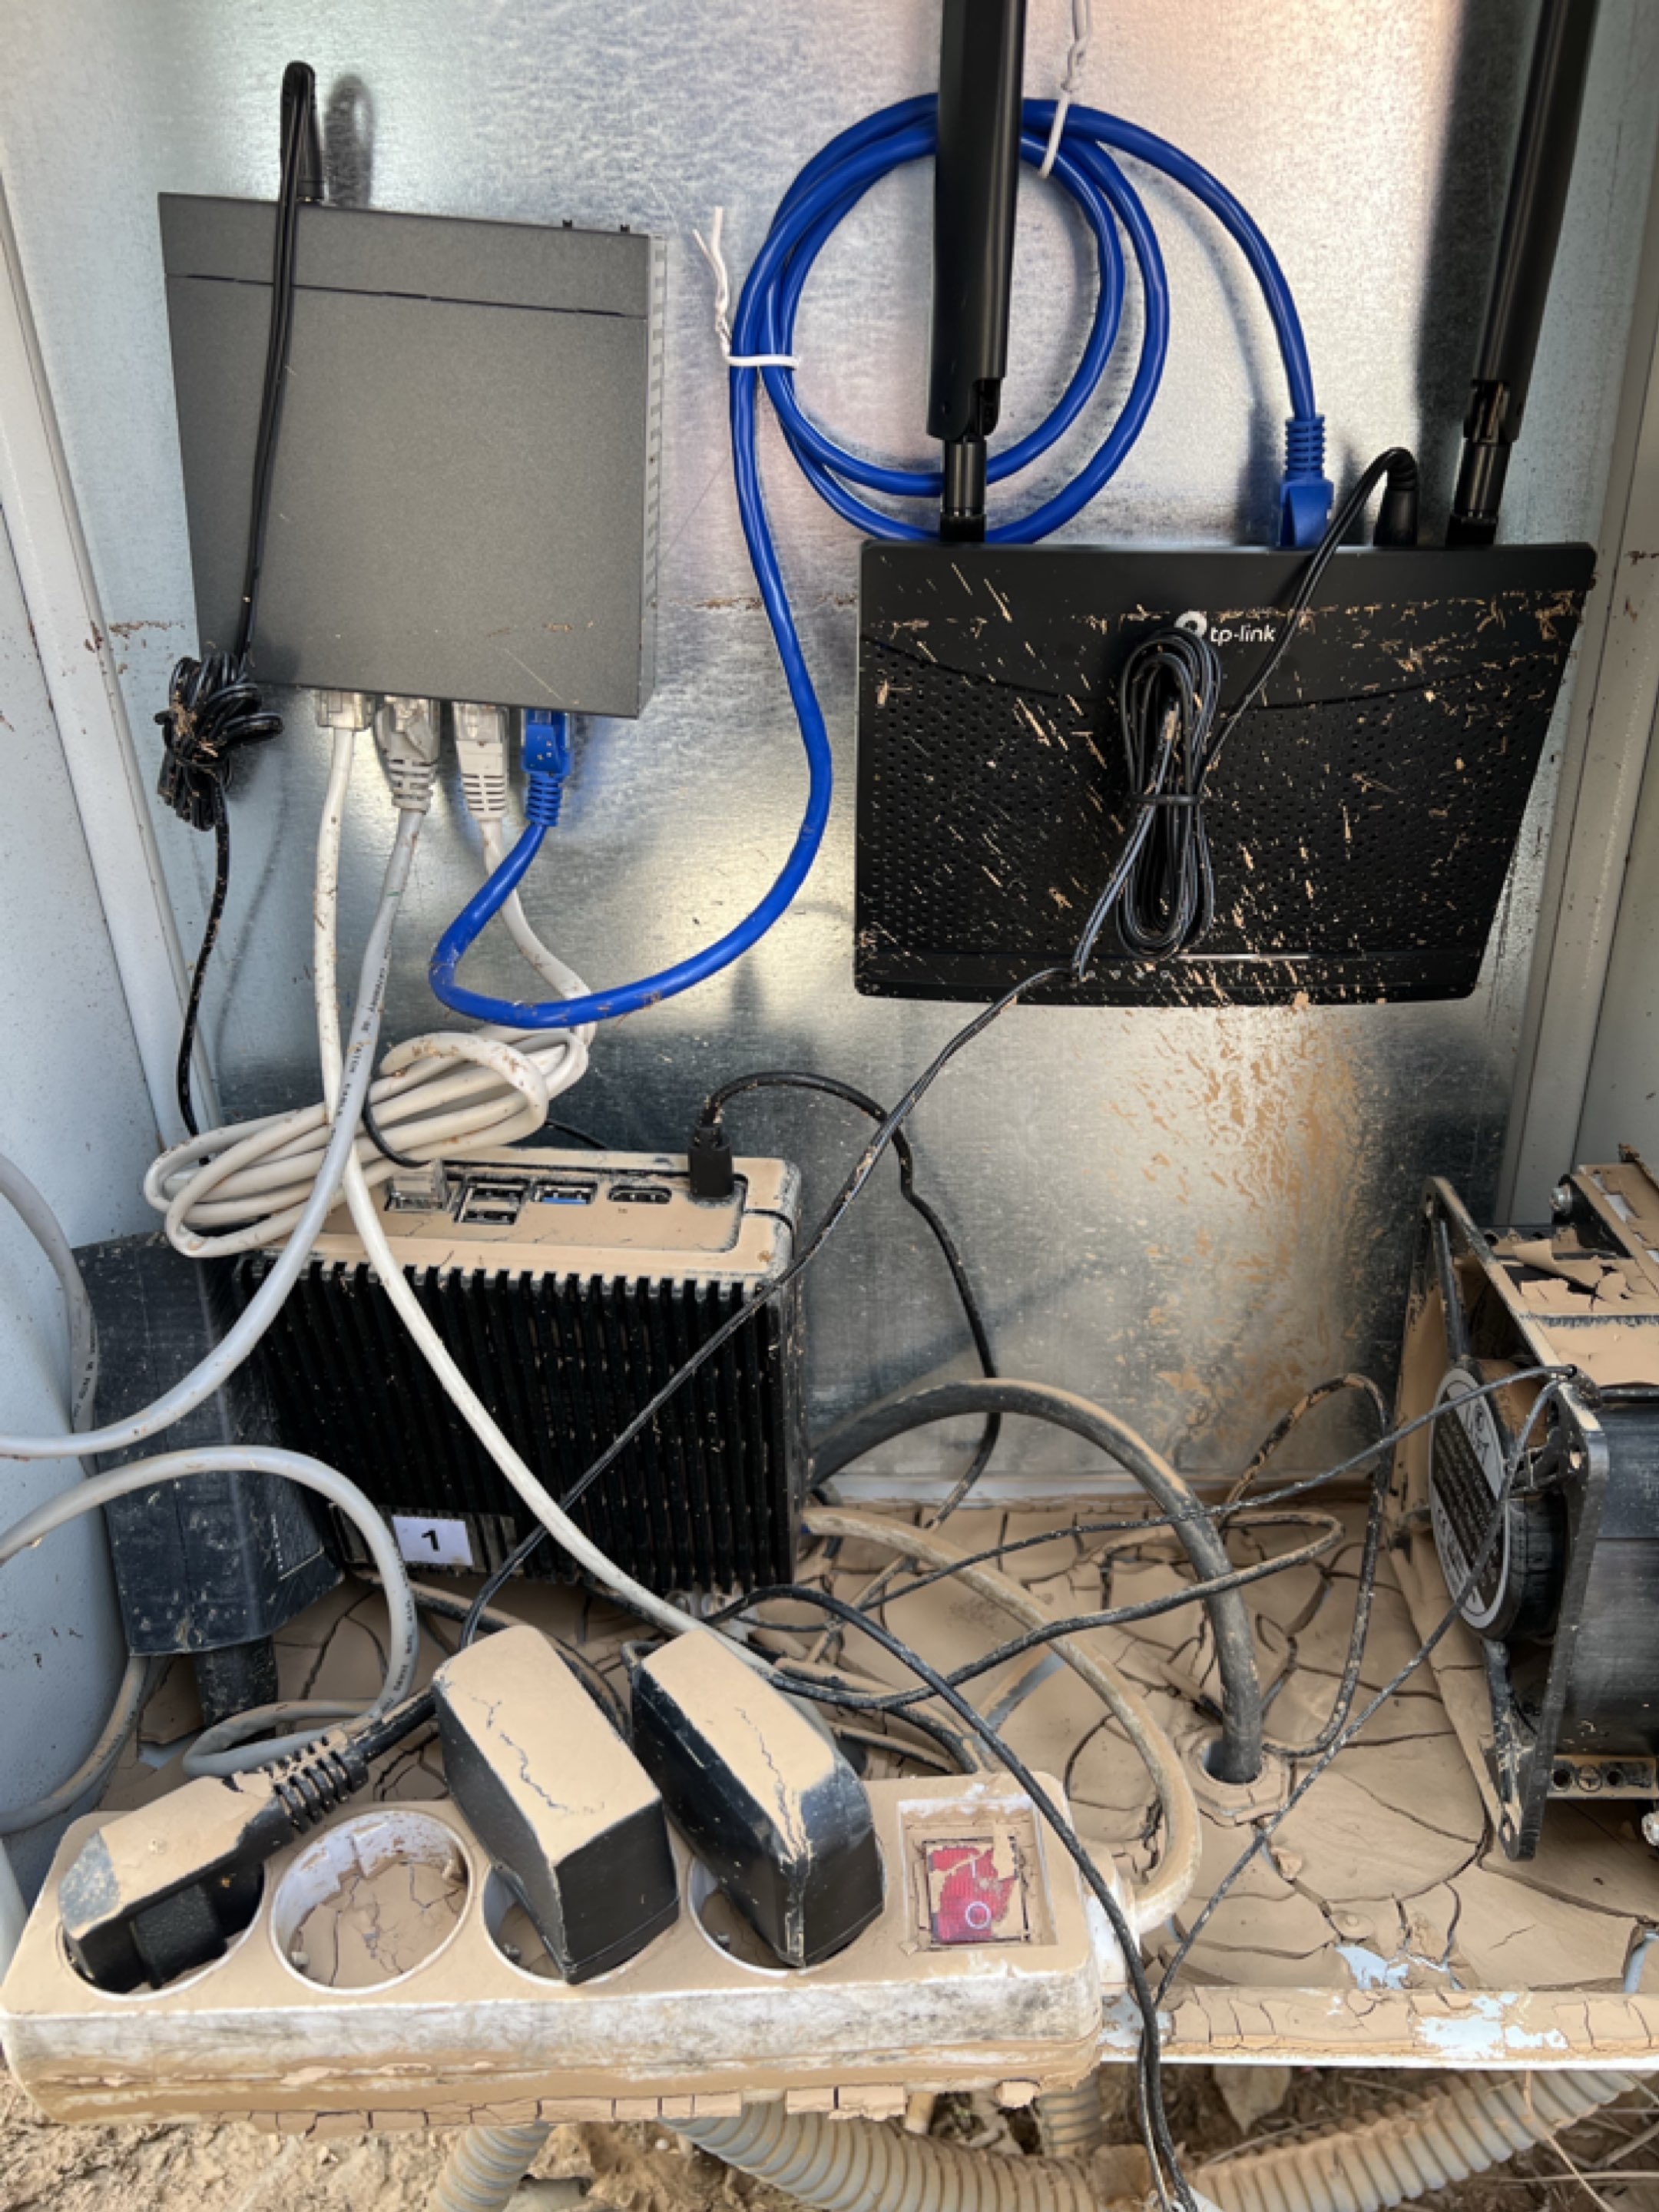
\includegraphics{dana.jpg}
    \caption{Dana weather effects on the system in one of the communities in Valencia, September 2024}\label{fig:dana}
\end{figure}

Camera performance was notably affected by varying weather conditions. Direct sunlight caused glare issues that impacted license plate recognition accuracy, while heavy rain sometimes triggered false readings as water made the lense blurry \cref{fig:wet_camera}. These challenges were addressed through the installation of protective shields and the refinement of the recognition algorithms to account for adverse weather conditions. 

\begin{figure}
        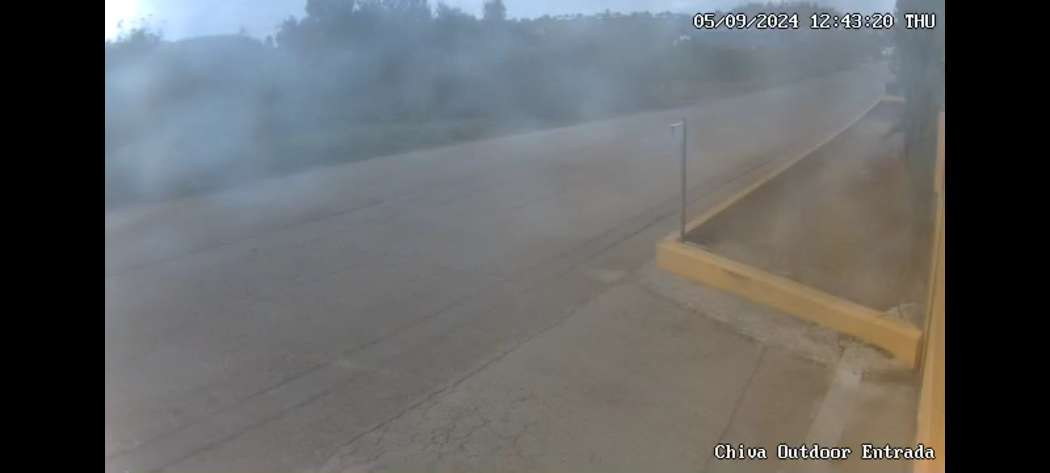
\includegraphics{empanado.jpg}
    \caption{Water leakage inside a camera making the image blurry}\label{fig:wet_camera}
\end{figure}

\section{Community-Specific Adaptations}

Different communities presented unique infrastructure requirements that necessitated system adaptations. Several communities required dual garage door configurations to manage separate entry and exit points. This led to the development of enhanced traffic flow management algorithms and modified hardware setups to coordinate multiple access points effectively. 

The installation process revealed varying electrical infrastructure across communities, requiring custom solutions for power delivery and surge protection. In older buildings, existing wiring needed to be carefully evaluated and sometimes upgraded to support the system's power requirements while maintaining safety standards.




\oldpart{Conclusions}\label{part:conclusions}

\chapter{Conclusions}\label{ch:conclusions}

While this thesis presentes the design, implementation, and testing of a distributed parking management system tailored for multi-community deployment, it establishes the basic architecture to be applied to other \gls{iot} solutions with edge computing and storage requirements. The project addresses limitations in existing systems by focusing on scalability, reliability, and adaptability, aligning with the goals of next-generation smart cities. 

Following the methodology outlined in \cref{ch:implementation}, the system was successfully deployed in ten communities around Valencia. The deployment has been running for six months. The system has processed thousands of entries and exits and has proven to be stable and reliable. 

Throughout the deployment, the system has undergone updates to meet specific community requirements. A configuration page was implemented to allow community administrators to manage settings such as parking limits, access permissions, and camera configurations. ML detection was improved to adapt to changes in environmental factors and improve the reliability of the system. A mobile app was released with basic functionalities to the users to interact with the system. A backup system was built and deployed to protect the database of the community to prevent data loss. A system to remotely update the different terminals has been developed. 

The implemented system demonstrated the feasibility of a distributed architecture for parking management, capable of operating autonomously within individual communities while maintaining centralized monitoring and control. The results of the project demonstrate the potential of the system to optimize parking space utilization, reduce traffic congestion, and enhance the overall urban experience.

\chapter{Future work}\label{ch:future_work}

\todo{write this chapter}

add that to change the db to a nosql for the users and keep the sql for the records

use prisma for the db

\chapter{Socio-economic environment}\label{ch:socio_economic_environment}

The widespread adoption of automated parking management systems is transforming urban environments and the economy, offering significant benefits while also presenting challenges. This chapter examines the socio-economic factors influencing the deployment of these systems, particularly in residential communities. It explores the potential advantages, obstacles, and financial implications of integrating this technology across urban areas.

\section{Social Impact}

Automated parking management systems have gained popularity due to their efficiency and ability to optimize space utilization, revolutionizing urban planning and mobility. Their capacity to reduce traffic congestion and improve parking availability can greatly enhance urban living conditions. For example, sensor-based systems can guide drivers to available parking spots, reducing time spent searching and lowering emissions. The project demonstrated how these systems can provide real-time occupancy data, aiding both residents and visitors in finding parking more efficiently.

In densely populated urban areas, automated parking systems facilitate better use of limited space. This capability not only improves the quality of life for residents but also contributes to more sustainable urban development by maximizing the use of available land.

However, privacy and data security remain concerns. The extensive data collection by these systems raises issues of surveillance and personal data protection, underscoring the need for clear regulations and ethical guidelines, as discussed in the regulatory framework chapter.

\section{Economic Impact}

The economic benefits of adopting automated parking management systems are substantial, with the potential to boost urban efficiency and drive innovation. For property managers and urban planners, these systems enable more efficient use of space, potentially increasing property values and reducing operational costs associated with parking management.

Despite these advantages, the costs of implementing automated parking systems (e.g., installation, training, maintenance, and upgrades) remain significant barriers for some communities and smaller property management companies. Moreover, the need for technical expertise and the risk of system failures can increase operational expenses.

\section{Environmental Impact}

Automated parking management systems can positively impact the environment by reducing traffic congestion and associated emissions. By guiding drivers directly to available spots, these systems minimize the time vehicles spend idling or circling in search of parking, contributing to lower air pollution and fuel consumption in urban areas.

Nonetheless, the environmental costs of manufacturing and disposing of electronic components must be considered. The production of sensors, cameras, and other hardware components can be resource-intensive. Sustainable design practices and proper e-waste management are necessary to mitigate these effects.

\section{Planning}

The project was structured into distinct phases, each with specific activities and tasks, as illustrated in \cref{fig:planning}. The timeline for these phases was planned on a weekly basis, detailing the progression of activities from initial research to final deployment. The first month and a half of the project was dedicated to understanding the problem, reviewing relevant literature, exploring the necessary tools, and configuring them for our specific needs. This initial phase, encompassing research and planning, required a significant time investment due to the complexities and documentation gaps associated with certain tools like AWS or hardware integration. The subsequent five months were focused on development of the system and the final three months to writing the final document.

\begin{figure}
    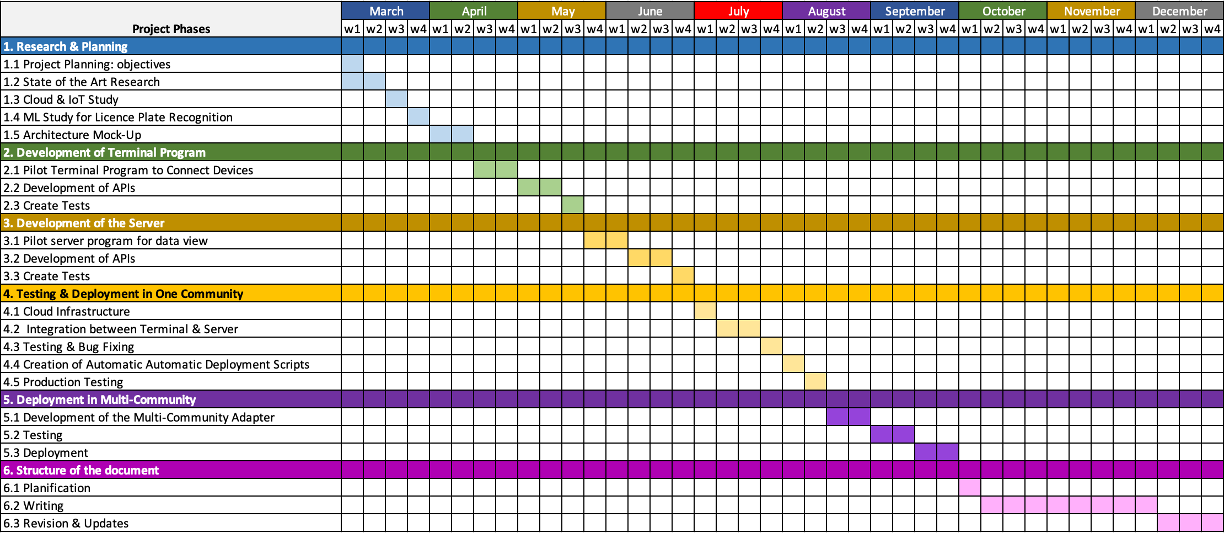
\includegraphics{planning.png}
    \caption{Gantt Chart for the Project Planning}\label{fig:planning}
\end{figure}

\section{Budget Analysis}

The cost of implementing automated parking management systems is a significant consideration for many communities. The analysis includes a detailed assessment of hardware components, software, maintenance, and other relevant expenses.

\cref{tab:hardware_costs_physical_components} details hardware costs for terminals, cameras, and networking equipment costs and other expenses for each community. The total cost for these physical components is estimated at 621 \euro\ per community. However, it is worth noting that for this project, 10 different communiteis have been installed totaling to 6210 \euro\ for the physical components. Moreover, in \cref{tab:costs_software_components} the cost of the software components are included totaling to 30 \euro. Moreover, the human costs associated to this project, refer to \cref{tab:human_costs}, amount to 13900 \euro.

For this project, the total cost would amount to 20140 \euro, which includes the necessary hardware and software for a typical residential community and the human labor costs. However, it's important to note that this does not account for installation and long-term maintenance costs or potential upgrades, which are essential for the system's longevity and effectiveness.

In conclusion, while automated parking management systems hold significant promise for urban areas and residential communities, careful consideration of social, economic, and environmental factors is essential. Addressing these challenges with appropriate regulations and sustainable practices will maximize their potential benefits in creating more livable and efficient urban spaces.

\begin{table}[H]
	\begin{tabular}{ l l r r }
		\toprule
		\textbf{Item}               & \textbf{Model}                                & \textbf{Quantity} & \textbf{Cost (\euro)} \\
		\midrule
		Edge Computer               & NVIDIA Jetson Nano \autocite{reComputerJ1010} & 1                 & 220                   \\
		Cameras                     & Reolink RLC-811A \autocite{ReolinkRLC811A}    & 2                 & 166                   \\
		Router                      & TP-Link AC1200 \autocite{TPLinkArcherMR600}   & 1                 & 85                    \\
		Reles                       &                                               & 1                 & 10                    \\
		Ethernet Cables             & Cat 6 30 meters                               & 1                 & 20                    \\
		4G SIM Card                 & Orange Prepaid SIM Card (1 month)             & 1                 & 10                    \\
		Boxes, power supplies, etc. &                                               & 1                 & 100                   \\
		\midrule
		\textbf{Total}              &                                               &                   & 621                   \\
		\bottomrule
	\end{tabular}
	\caption{Hardware costs for the physical components for one community.}\label{tab:hardware_costs_physical_components}
\end{table}

\begin{table}[H]
	\begin{tabular}{ l l l r }
		\toprule
		\textbf{Item}  & \textbf{Model}                           & \textbf{Quantity} & \textbf{Cost (\euro)} \\
		\midrule
		Server         & Amazon Web Services Deployment (1 month) & 1                 & 30                    \\
		\midrule
		\textbf{Total} &                                          &                   & 30                    \\
		\bottomrule
	\end{tabular}
	\caption{Costs for the software components and maintenance.}\label{tab:costs_software_components}
\end{table}

\begin{table}[H]
    \begin{tabular}{ l l l r }
        \toprule
		\textbf{Item}  & \textbf{Model}                           & \textbf{Quantity} & \textbf{Cost (\euro)} \\
        \midrule
        Personal Computer & Macbook Air & 1 & 1600  \\
        Junior Engineer Hours & 15 \euro/h & 500 & 7500 \\
        Senior Engineer Hours & 60 \euro/h & 40 & 2400 \\
        Electricity, labs, climate control, management, etc. & & & 2040 \\
        \midrule
        \textbf{Total} & & & 13900 \\
        \bottomrule
    \end{tabular}
    \caption{Human costs.}\label{tab:human_costs}
\end{table}

\chapter{Regulatory Framework}\label{ch:regulatory_framework}

The regulatory framework governing smart cities in Europe is primarily based on the data protection provisions outlined in the \gls{gdpr}. This is largely because these systems employ surveillance technologies such as cameras that monitor public spaces, and they handle sensitive personal data, including individuals' identification numbers and contact information. Additionally, the integration of technologies such as the \gls{iot}, \gls{ai}, and data analytics has necessitated robust legal mechanisms to address privacy, security, and ethical considerations.

\section{Applicable Legislation}

The implementation and operation of smart city technologies in the European Union must adhere to a range of legislative measures that regulate data privacy, electronic communications, and emerging technologies. Chief among these is the \gls{gdpr}, but other complementary regulations and directives are also critical in shaping the regulatory landscape.

\subsection{General Data Protection Regulation (GDPR)}

The \gls{gdpr} \autocite{eu-679-2016}, also known as the Regulation (EU) 2016/679 and enacted in 2016, provides a comprehensive framework for the protection of personal data within the European Union. Its principles of transparency, accountability, and data minimization serve as the cornerstone of privacy and data protection.

Under \gls{gdpr}, smart city systems are required to obtain explicit consent from individuals before collecting or processing their personal data. Furthermore, data controllers must implement privacy-by-design and privacy-by-default principles, ensuring that data protection is an integral aspect of technological development. Smart cities must also conduct Data Protection Impact Assessments for projects involving high-risk data processing, such as large-scale surveillance or facial recognition.

\subsection{Data Retention Policies}

Smart city technologies often rely on continuous data collection through sensors, cameras, and connected devices. The \gls{gdpr} mandates that data should only be retained for as long as necessary to fulfill its intended purpose. To comply, smart city operators must establish robust data retention and deletion policies. Automated systems are frequently employed to enforce these policies, ensuring that unnecessary data is securely deleted to minimize privacy risks and reduce storage costs.

\subsection{ePrivacy Directive}

The ePrivacy Directive (Directive 2002/58/EC) \autocite{eu-58-2002}, commonly known as the "Cookie Law," governs the confidentiality of communications and the processing of electronic communications data. While initially designed for traditional telecommunications, its principles are increasingly relevant to smart city applications, such as real-time traffic monitoring and public Wi-Fi networks.

Under this directive, consent is required for the use of tracking technologies and location-based services, ensuring that users are aware of how their data is being utilized. The ongoing transition to the ePrivacy Regulation aims to enhance these protections and provide greater harmonization across member states.

\subsection{Directive on Security of Network and Information Systems (NIS 2 Directive)}

The \gls{nis} 2 Directive \autocite{eu-1148-2016}, adopted in 2016, focuses on the security of critical infrastructure and essential services, including those used in smart cities. It requires operators of essential services to implement risk management measures and report significant cybersecurity incidents to relevant authorities. For smart cities, this includes safeguarding critical systems such as transportation networks, energy grids, and communication systems against cyber threats.

\subsection{Artificial Intelligence Act}

The Artificial Intelligence Act \autocite{eu-1689-2024}, which came into force on 1 August 2024, establishes a common regulatory and legal framework for \gls{ai} across the European Union. Its provisions will be implemented gradually over the following 6 to 36 months. The Act classifies AI systems into categories based on risk—ranging from minimal to unacceptable—and imposes specific requirements on high-risk AI applications.

For smart cities, the Act directly impacts technologies such as AI-driven surveillance systems, autonomous transportation, and automated decision-making tools. These applications must adhere to stringent requirements, including transparency, accountability, and mandatory human oversight. The Act ensures that AI technologies in smart cities are deployed ethically and align with EU values, particularly with respect to fundamental rights and safety.

\section{Regulatory Challenges and Implications}

The evolving nature of smart city technologies presents significant challenges for regulatory compliance. These challenges include the integration of multiple technologies such as \gls{iot}, \gls{ai}, and data analytics, which often involve cross-border data flows and raise questions about jurisdiction and enforcement. Furthermore, the pace of technological innovation frequently outstrips the development of regulatory frameworks, creating gaps that may expose users to privacy and security risks.

Ensuring compliance with a wide array of legislative measures requires substantial investment in training and capacity-building for smart city administrators. Policymakers and industry stakeholders must collaborate to establish clear guidelines that address emerging issues while balancing innovation and the protection of fundamental rights.

\section{Conclusion}

The regulatory landscape for smart cities in Europe, underpinned by the \gls{gdpr}, the ePrivacy Directive, the \gls{nis} 2 Directive, the Artificial Intelligence Act, and other complementary legislation, provides a robust foundation for ethical and secure technological deployment. As the European Union continues to refine its regulatory framework, smart cities are poised to achieve a harmonious balance between technological advancement and the protection of individual rights. By prioritizing compliance, transparency, and accountability, European smart cities can serve as global exemplars of ethical innovation.



\blankpage%
\printbibliography%

\end{document}
